% !TEX program = xelatex
% ============================================================
%  全国大学生数学建模竞赛 (CUMCM) LaTeX 通用论文模板
%  编译方式: XeLaTeX
% ============================================================
\documentclass[12pt,a4paper]{ctexart}

% ======================== 宏包加载 ========================
\usepackage[top=2.5cm, bottom=2.5cm, left=2.8cm, right=2.8cm]{geometry}
\usepackage{amsmath, amssymb, amsthm}
\usepackage{graphicx}
\usepackage{float}
\usepackage{subcaption}
\usepackage{booktabs}
\usepackage{array}
\usepackage{multirow}
\usepackage{longtable}
\usepackage{xcolor}
\usepackage{hyperref}
\hypersetup{
    colorlinks=true,
    linkcolor=blue!70!black,
    citecolor=green!50!black,
    urlcolor=blue!60!black
}
\usepackage{listings}
\lstset{
    basicstyle=\small\ttfamily,
    breaklines=true,
    frame=single,
    numbers=left,
    numberstyle=\tiny\color{gray},
    keywordstyle=\color{blue},
    commentstyle=\color{green!60!black},
    stringstyle=\color{red!70!black},
    tabsize=4
}

\usepackage{setspace}
\onehalfspacing
\usepackage{enumitem}
\setlist{nosep, leftmargin=2em}
\usepackage{titlesec}
\usepackage{caption}
\usepackage{bm}
\usepackage{mathtools}
\usepackage{indentfirst}

% ======================== 字体设置 ========================
\setCJKmainfont{SimSun}[BoldFont=SimHei, ItalicFont=KaiTi]
\setCJKsansfont{SimHei}
\setCJKmonofont{FangSong}
\setmainfont{Times New Roman}

% ======================== 首行缩进 ========================
\setlength{\parindent}{2em}

% ======================== 编号格式 ========================
\renewcommand{\thesection}{\chinese{section}、}
\renewcommand{\thesubsection}{\arabic{section}.\arabic{subsection}}
\renewcommand{\thesubsubsection}{\arabic{section}.\arabic{subsection}.\arabic{subsubsection}}

% ======================== 标题格式 ========================
\titleformat{\section}
  {\centering\heiti\zihao{-3}\bfseries}
  {\thesection}{0em}{}
\titlespacing*{\section}{0pt}{1.5ex plus .5ex minus .2ex}{1.0ex plus .2ex}

\titleformat{\subsection}
  {\heiti\zihao{4}\bfseries}
  {\thesubsection}{1em}{}
\titlespacing*{\subsection}{0pt}{1.2ex plus .4ex minus .2ex}{0.8ex plus .2ex}

\titleformat{\subsubsection}
  {\heiti\zihao{-4}\bfseries}
  {\thesubsubsection}{1em}{}
\titlespacing*{\subsubsection}{0pt}{1.0ex plus .3ex minus .1ex}{0.6ex plus .1ex}

% ======================== 定理环境 ========================
\theoremstyle{definition}
\newtheorem{definition}{定义}[section]
\newtheorem{assumption}{假设}[section]
\theoremstyle{plain}
\newtheorem{theorem}{定理}[section]
\newtheorem{lemma}{引理}[section]
\newtheorem{proposition}{命题}[section]
\newtheorem{corollary}{推论}[section]
\theoremstyle{remark}
\newtheorem{remark}{注}[section]

% ======================== 自定义命令 ========================
\renewenvironment{abstract}
  {\begin{center}\heiti\zihao{-3}\bfseries 摘\quad 要\end{center}\zihao{-4}\songti}
  {\par\vspace{1em}}

\newcommand{\keywords}[1]{%
  \par\noindent\textbf{关键词：}#1}

\newenvironment{symboltable}
  {\begin{center}\zihao{5}\begin{tabular}{>{\centering\arraybackslash}p{3.5cm} p{7.5cm} >{\centering\arraybackslash}p{1.5cm}}
  \toprule
  \textbf{符号} & \textbf{含义} & \textbf{单位} \\
  \midrule}
  {\bottomrule\end{tabular}\end{center}}

\newcommand{\step}[1]{\par\noindent\textbf{Step #1}\quad}

% ============================================================
\begin{document}
\pagestyle{plain}

\begin{center}
{\zihao{-2}\heiti\bfseries 基于约束凝聚聚类与模拟退火的管道最优铺设方案}
\end{center}
\vspace{1em}

% ======================== 摘要 ========================
\setcounter{page}{1}
\pagenumbering{arabic}

\begin{abstract}
\setlength{\parindent}{2em}

\indent 本文针对某地区180个供水点的两级输水管网优化问题，综合考虑二级管道30公里长度的约束与管道造价的差异性，构建了\textbf{带长度约束的多级设施选址与网络设计数学模型}。基于\textbf{约束感知凝聚聚类}、\textbf{加权评分选址}、\textbf{最小生成树组网}及\textbf{模拟退火}全局寻优的共分四个阶段的求解策略，有效解决了\textbf{NP-Hard}组合优化难题并实现了总建设费用最小化。

\indent 针对该两级管网优化问题，本文基于\textbf{Delaunay三角剖分}性质将原节点图从完全图降至稀疏图，在保证不丢失最小生成树边的前提下显著提升后续聚类与寻优效率。在此基础上，建立了\textbf{带长度约束的两级设施选址与网络设计数学模型}，并设计了\textbf{``约束感知凝聚聚类——加权评分选址——MST组网——模拟退火全局寻优''}的四阶段求解策略：通过嵌入最小生成树长度校验的聚类算法确保节点簇的划分严格满足管道长\textbf{30公里}的硬约束；构建兼顾二级管网覆盖质量与一级管网连通成本的加权评分函数来平衡成本，以确定一级供水站位置；分别生成I型骨干网与II分支网的最小生成树拓扑；引入\textbf{模拟退火算法}并通过边界节点漂移、站址替换及节点簇分裂合并三种方法突破贪心算法的局限性进行全局寻优。最终求得总费用为\textbf{35692.95万元}的最优方案，其中I型管道总长\textbf{139.66公里}，II型管道总长\textbf{396.91公里}，所有二级供水站节点簇的管网里程均严格低于\textbf{30公里}且容量利用率普遍超过\textbf{90\%}，较最初得到的解降低\textbf{2.68\%}。
\end{abstract}

\keywords{两级管网优化；带容量约束设施选址；约束凝聚聚类；最小生成树；模拟退火}
\newpage

% ======================== 目录（可选，取消注释启用） ========================
% \newpage
% \tableofcontents
% \newpage
% ============================================================
% 正文部分开始 (请将其粘贴至您的 .tex 文件中摘要及关键词之后)
% ============================================================

\section{问题重述}
\subsection{问题背景}
区域集中供水工程是保障地方水资源合理配置与民生需求的关键基础设施。区域集中供水工程需为180个分散供水点设计两级输水管网。在中心站A处建立水源枢纽，采用“中心站—一级站—二级站”层级拓扑：中心站至一级站铺设I型管道DN250，一级站至二级站铺设II型管道DN125。两类管道的材料成本与铺设费用存在显著差异。此外，受一级站设备增压功率的物理限制，从单一一级站出发铺设的II型管道总里程存在30公里的硬性上限。如何在满足所有工程约束的前提下，科学遴选一级站址并优化管网拓扑，以实现总建设费用的最小化，是本规划面临的核心难题。

\subsection{问题提出}
现已知中心站A与180个供水点的精确空间坐标，以及两类管道的单位造价及铺设费用。本文需要解决的核心问题是：综合考虑上述工程约束与建设成本，建立带长度约束的多级设施选址与网络设计数学模型，科学确定一级供水站的最优选址方案以及I型与II型管道的连接拓扑结构。在确保所有供水点被有效覆盖且满足30公里二级管网里程硬约束的前提下，使得整个管网系统的总铺设费用达到最小，并给出具体的选址坐标、管道分布长度及最小费用结果。
\section{问题分析}
本问题的本质是一个\textbf{带长度约束的两级设施选址问题}与\textbf{多层级网络设计问题}的耦合。由于一级站的候选方案数高达 $2^{180}-1$，该问题属于典型的NP-Hard组合优化问题。在180个节点的规模下，传统的精确算法难以处理如此庞大的计算量，以至于无法在有效时间内求解这个问题。因此，必须从图论与空间几何的视角对问题进行简化与解耦分析。

\subsection{多级管网拓扑结构与约束机制分析}
管网设计可抽象为在由181个节点构成的完全图上选取边子集以构建连通树结构的过程，题目的工程上的约束对网络拓扑提出了严格的限制。一方面，管网呈现明确的两级层级特征，I型管道构成连接中心站与所有一级站的骨干树，II型管道则构成连接一级站与其所属二级站的分支树。另一方面，受限于管道必须从供水站节点出发的施工要求，管网中禁止在管道中间任意点分支，这意味着网络结构必须是严格基于给定节点集的生成树，而无法引入额外的中间分支点。此外，30公里的二级管道长度硬约束是本题最核心的难点，该限制要求从任一一级站出发铺设的II型管道总里程不得超过30公里，从而将全局网络割裂为若干个以一级站为根的独立子树。这一特性使得节点聚类划分与求解管网拓扑问题难以分开，无法作为独立子问题分别求解，极大增加了问题的求解复杂度。
\subsection{空间受限下的聚类与选址策略分析}
针对30公里硬约束，常规聚类算法无法直接控制管网总长。为此，我们改进了凝聚层次聚类算法，使其具备约束处理能力，即把最小生成树长度校验嵌入每一次合并操作里。只有当两个簇合并后的最小生成树总长不超过30公里时，才允许合并。这一设计确保了所有产出簇天然满足容量限制，避免了无效搜索。
\subsection{启发式算法的全局优化分析}
前述聚类、选址与组网的贪心求解策略虽然计算效率高，但本质上属于局部搜索，极易陷入局部最优。例如有时将边界节点的归属进行微调可能带来全局成本的下降，而贪心策略往往无法发现此类需要暂时变差才能继续优化的路径。为此，本文引入模拟退火算法进行全局寻优。通过设计定制化的邻域算子，涵盖边界节点漂移、一级站址替换以及簇的分裂与合并，在严格满足30公里硬约束的可行域内，允许暂时接受成本更高的方案，从而有效跳出局部最优，逼近全局最优解。
\section{模型假设}
\begin{enumerate}[label=\arabic*.]
  \item 假设相邻两站间管道沿直线铺设，长度取欧氏距离，忽略地形起伏与地下障碍物对施工路线的影响。
  \item 假设管网结构为无向图上的树结构，不允许在管道中间任意点分支。
  \item 鉴于II型管道规格统一且缺乏流量数据，采用管道总物理长度作为功率负荷的线性指标来表现30公里约束，忽略末端流量差异导致的非线性水头损失波动。
  \item 依据题目给定统一单价参数，假设单位建设成本在规划区域内为常数，不考虑地质与土地性质差异导致的局部施工成本不同对管网拓扑结构决策的影响。
\end{enumerate}

\section{符号说明}
\begin{symboltable}
$V = \{0, 1, \ldots, 180\}$  & 节点全集，其中0为中心站A & -  \\
$(x_i, y_i)$  & 节点 $i$ 的二维空间坐标 & km  \\
$d_{ij}$  & 节点 $i, j$ 间的欧氏距离 & km  \\
$S \subseteq V \setminus \{0\}$  & 一级供水站集合（决策变量） & -  \\
$E_I, E_{II}$  & I型、II型管道边集 & -  \\
$L_I, L_{II}$  & I型、II型管道总长度 & km  \\
$c_I = 1291000$  & I型管道综合单价 & 元/km  \\
$c_{II} = 445000$  & II型管道综合单价 & 元/km  \\
$C_k$  & 第 $k$ 个供水簇（子树） & -  \\
$L_{MST}(C_k)$  & 簇 $C_k$ 的最小生成树总长 & km  \\
\end{symboltable}

\section{模型准备}
\subsection{说明节点空间分布特征与数据预处理}
管道网设计的本质是在完全图 $K_{181}$ 上选取边子集来构成树结构。首先读取181个节点的坐标，计算两两节点间的欧氏距离，得到 $181\times181$ 大小的对称距离矩阵 $D=[d_{ij}]$，共含 $\binom{181}{2}=16290$ 条候选边。

观察图一中180个供水点的空间分布，181个节点呈现多个自然聚集区域，如左下区域、中部密集区、右上区域及顶部散布区。这种节点之间的空间聚集性为先聚类、再选址、后组网的分治求解思路提供了几何直观上的支撑。

% 图1：供水点空间分布
\begin{figure}[H]
\centering
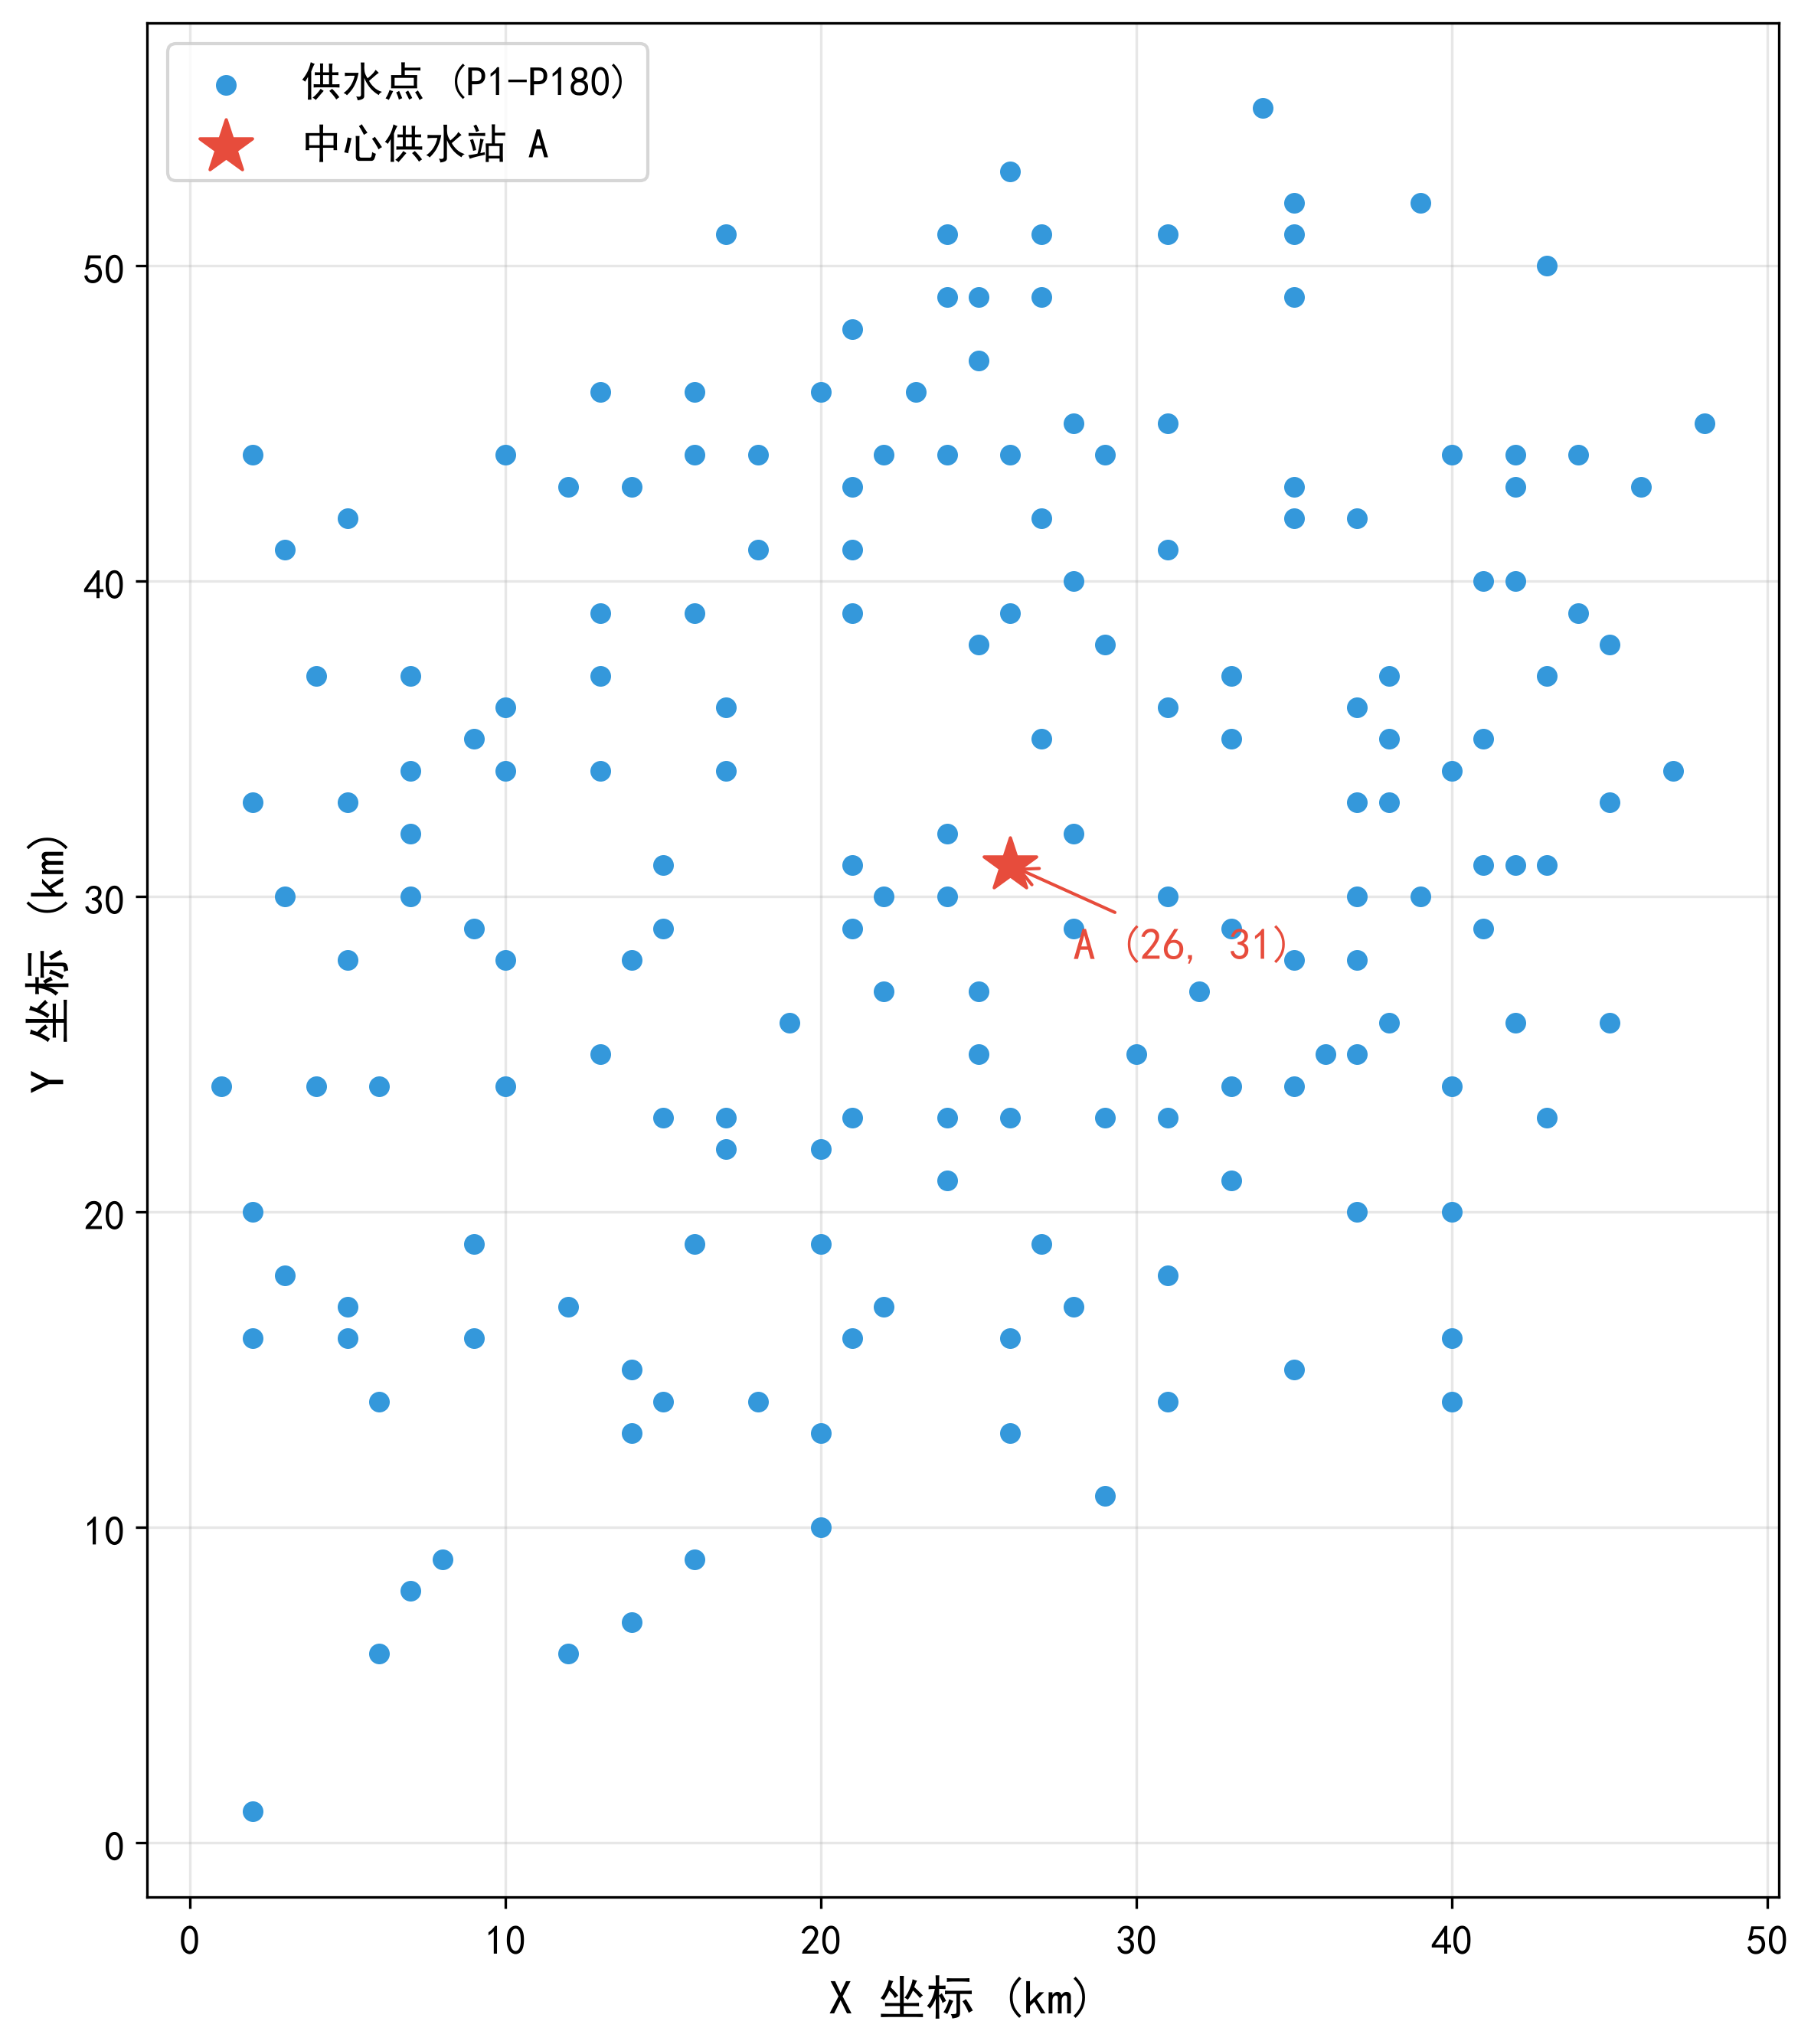
\includegraphics[width=0.7\textwidth]{figures/图1_供水点空间分布.png}
\caption{供水点与中心站A空间分布图}
\label{fig:spatial_dist}
\end{figure}


\subsection{基于Delaunay三角剖分方法的管道图简化}
为削减后续最优解搜索空间大小，利用Delaunay三角剖分法对候选边进行筛选。计算几何理论表明：欧氏点集的最小生成树必为其Delaunay图的子图。这意味着利用Delaunay三角剖分法剖分后的稀疏图依旧包含最优管道网所需的全部候选边，删去原图中的非最优边不损失整体的最优性。图\ref{fig:delaunay}展示了Delaunay剖分结果与全局MST的叠加关系，直观验证了MST的所有边均落在剖分后的稀疏图内。

% 图2：Delaunay三角剖分
\begin{figure}[H]
\centering
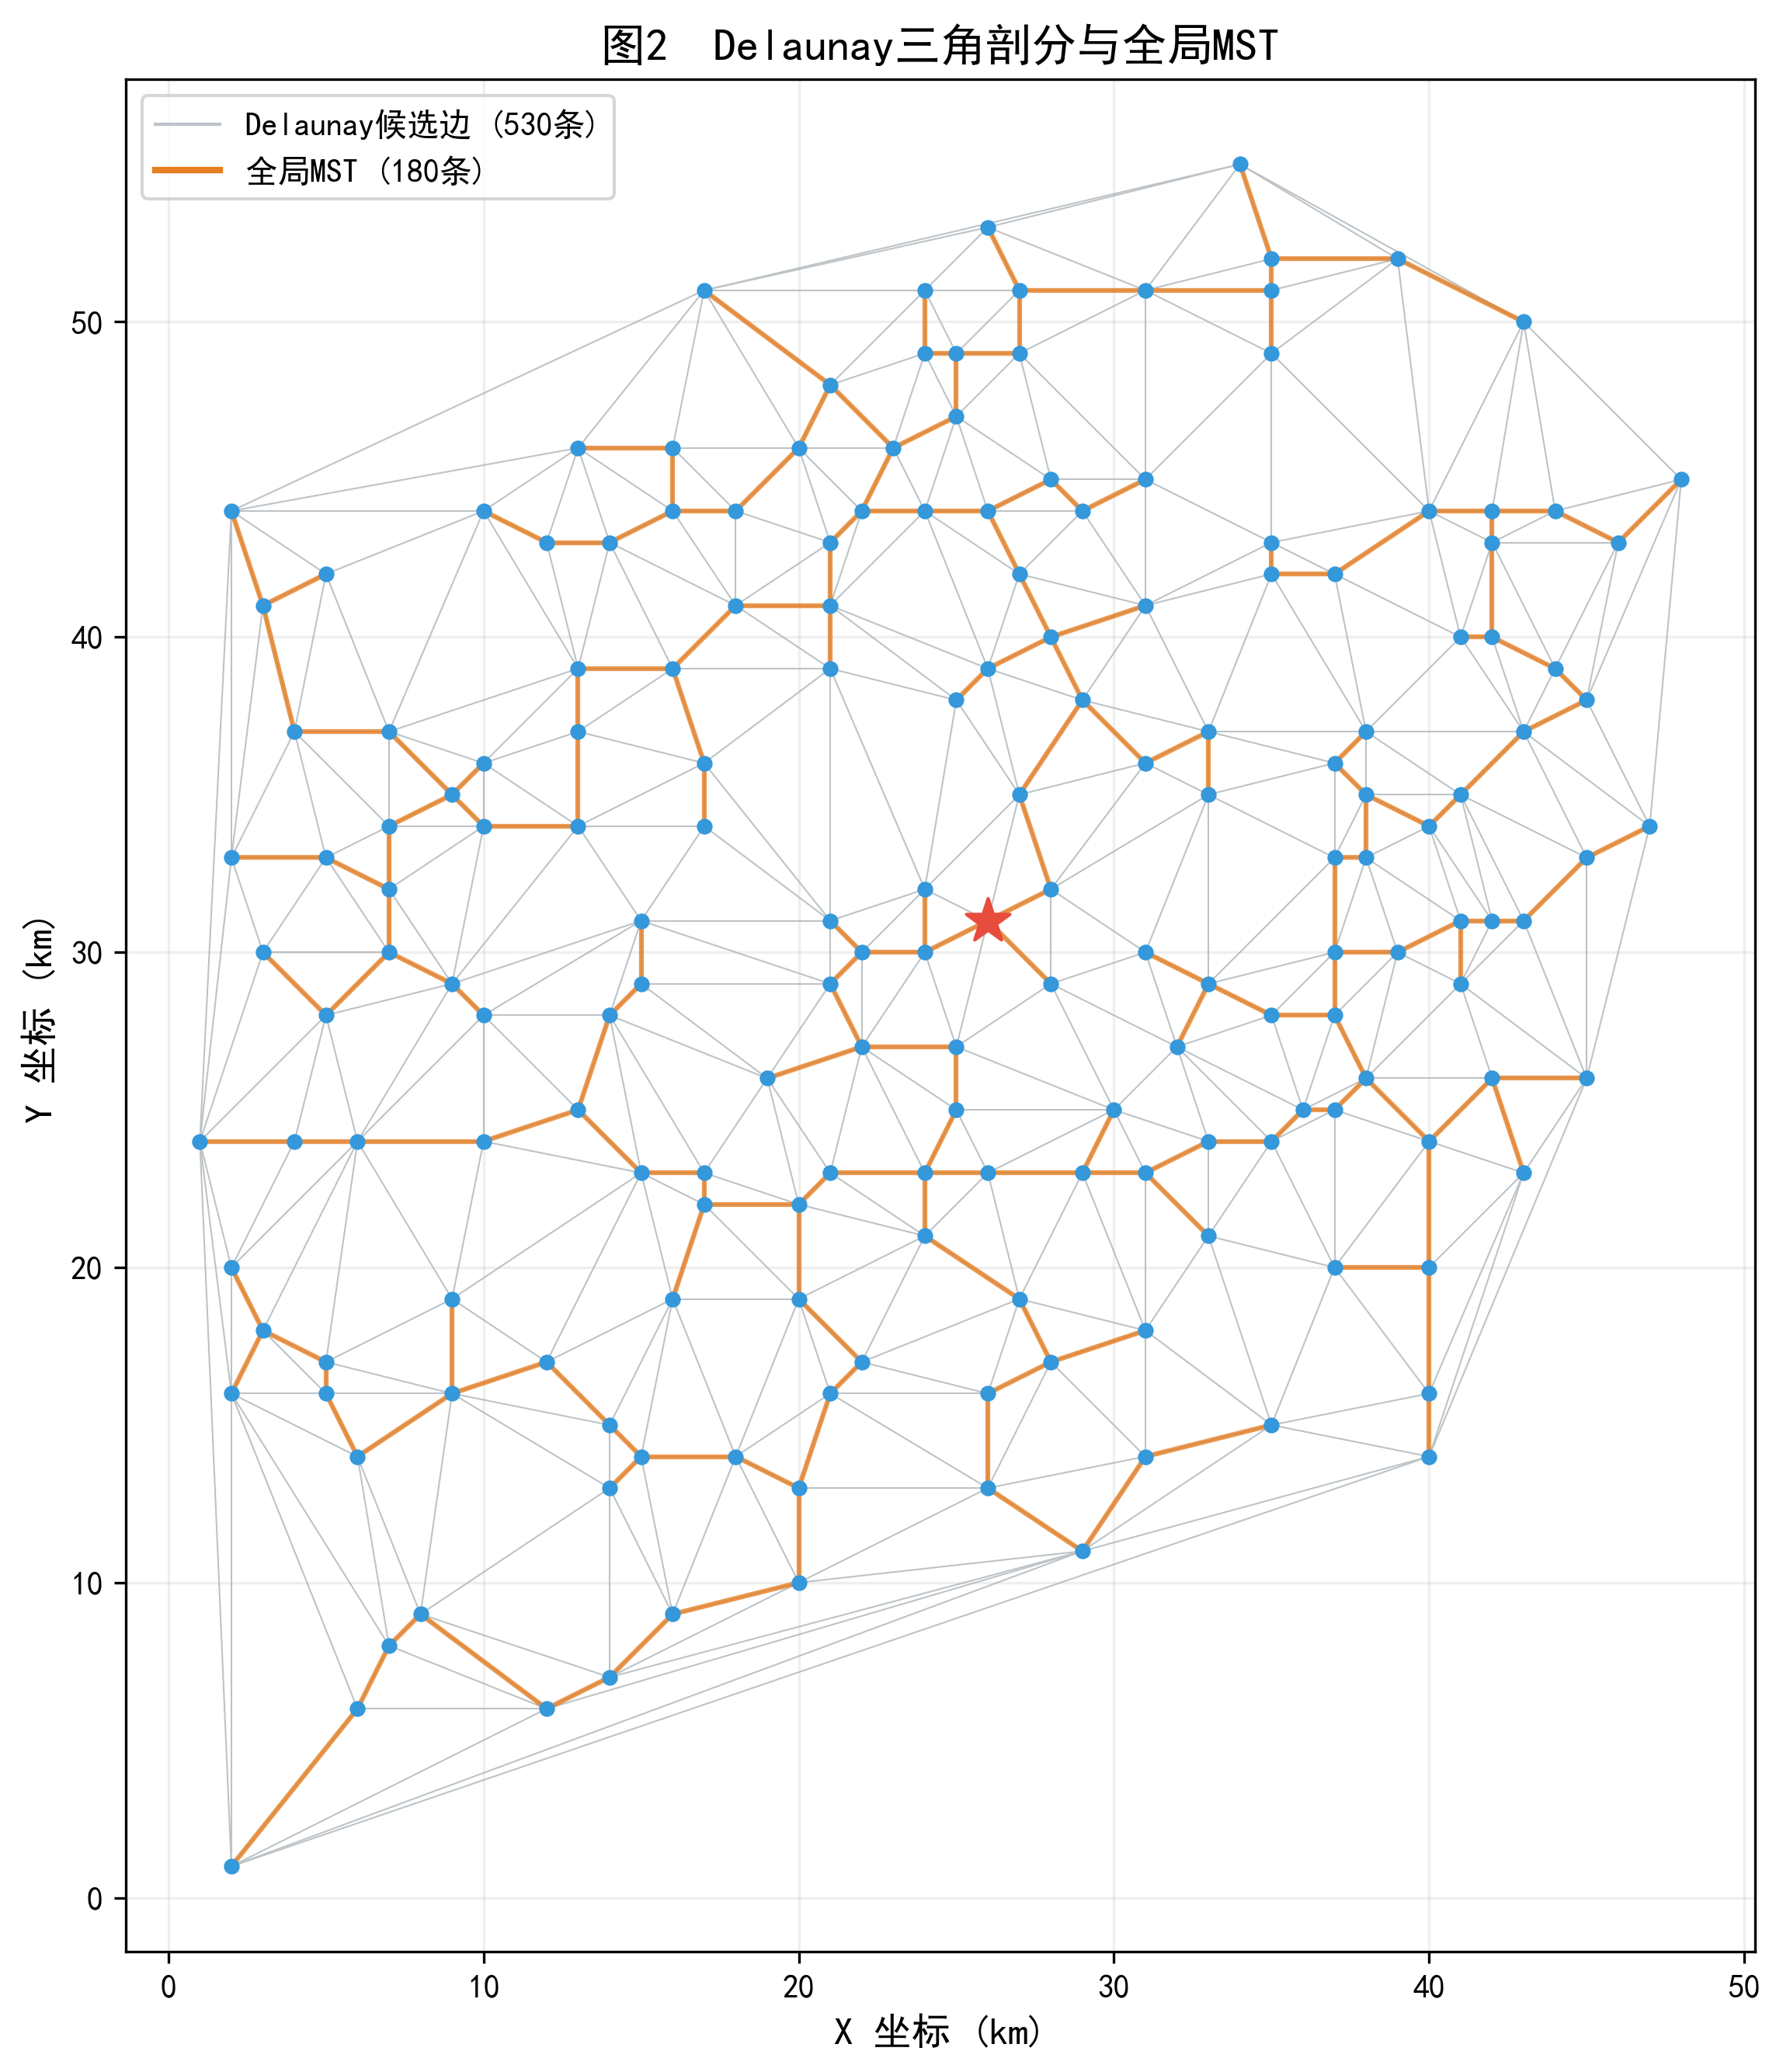
\includegraphics[width=0.7\textwidth]{figures/图2_Delaunay三角剖分.png}
\caption{Delaunay三角剖分候选边与全局最小生成树边集叠加图}
\label{fig:delaunay}
\end{figure}

\section{模型建立与求解}
\subsection{带容量约束的两级管网数学模型}
基于上述分析，建立如下非线性组合优化模型。
\subsubsection{目标函数}
以总铺设费用最小化为目标：
\begin{equation}
\min \; C_{total} = c_I \cdot L_I + c_{II} \cdot L_{II} = 1291000 \sum_{(i,j) \in E_I} d_{ij} + 445000 \sum_{(i,j) \in E_{II}} d_{ij}
\label{eq:obj}
\end{equation}

\subsubsection{约束条件}
\begin{itemize}
    \item \textbf{C1：}I型边集 $E_I$ 构成包含中心站A与所有一级站的连通树；每个II型子树 $E_{II}^{(k)}$ 构成包含对应一级站与簇内所有二级站的连通树。
    \item \textbf{C2：}中心站A仅与一级站相连，不直连二级站。
    \item \textbf{C3：}管道仅从供水站节点出发，边集端点必须属于 $V$，无额外点。
    \item \textbf{C4：}对每个一级站管辖的簇 $C_k$，其II型管道子树总边长不超过30公里：
    \begin{equation}
    \forall C_k: \sum_{(i,j) \in E_{II}^{(k)}} d_{ij} \le 30 \text{ (km)}
    \label{eq:capacity}
    \end{equation}
    \item \textbf{C5：}每个二级站仅连接一个一级站。
\end{itemize}

\subsection{基于30公里约束的空间受限聚类}
由于约束(\ref{eq:capacity})直接限制了簇内最小生成树的长度，本文设计了约束下的凝聚层次聚类算法。
\step{1}每个节点先自成一簇，形成180个仅含一个点的节点簇，节点簇内最小生成树长度为0。
\step{2}簇间距离采用，将两个簇之间的距离确定为两个簇中任意两点之间的最短距离：$d(C_a, C_b) = \min_{i\in C_a, j\in C_b} d_{ij}$。单链接准则倾向生成链状节点簇，与管道网络的树状拓扑结构较为契合。
\step{3}反复选取距离最近的节点簇对 $(C_a, C_b)$，计算合并后候选簇 $C_{trial} = C_a \cup C_b$ 的最小生产树的总长度 $L_{trial}$。若 $L_{trial} \le 30$ km，则接受合并；否则不合并该对节点，并将其标记为“不可合并”，继续尝试下一对节点。
\step{4}直至无任何簇对可在约束下合并。
算法终止后得到17个合适的节点簇，各簇空间分布及最小生成树长度如图\ref{fig:cluster}所示。

\begin{figure}[H]
\centering
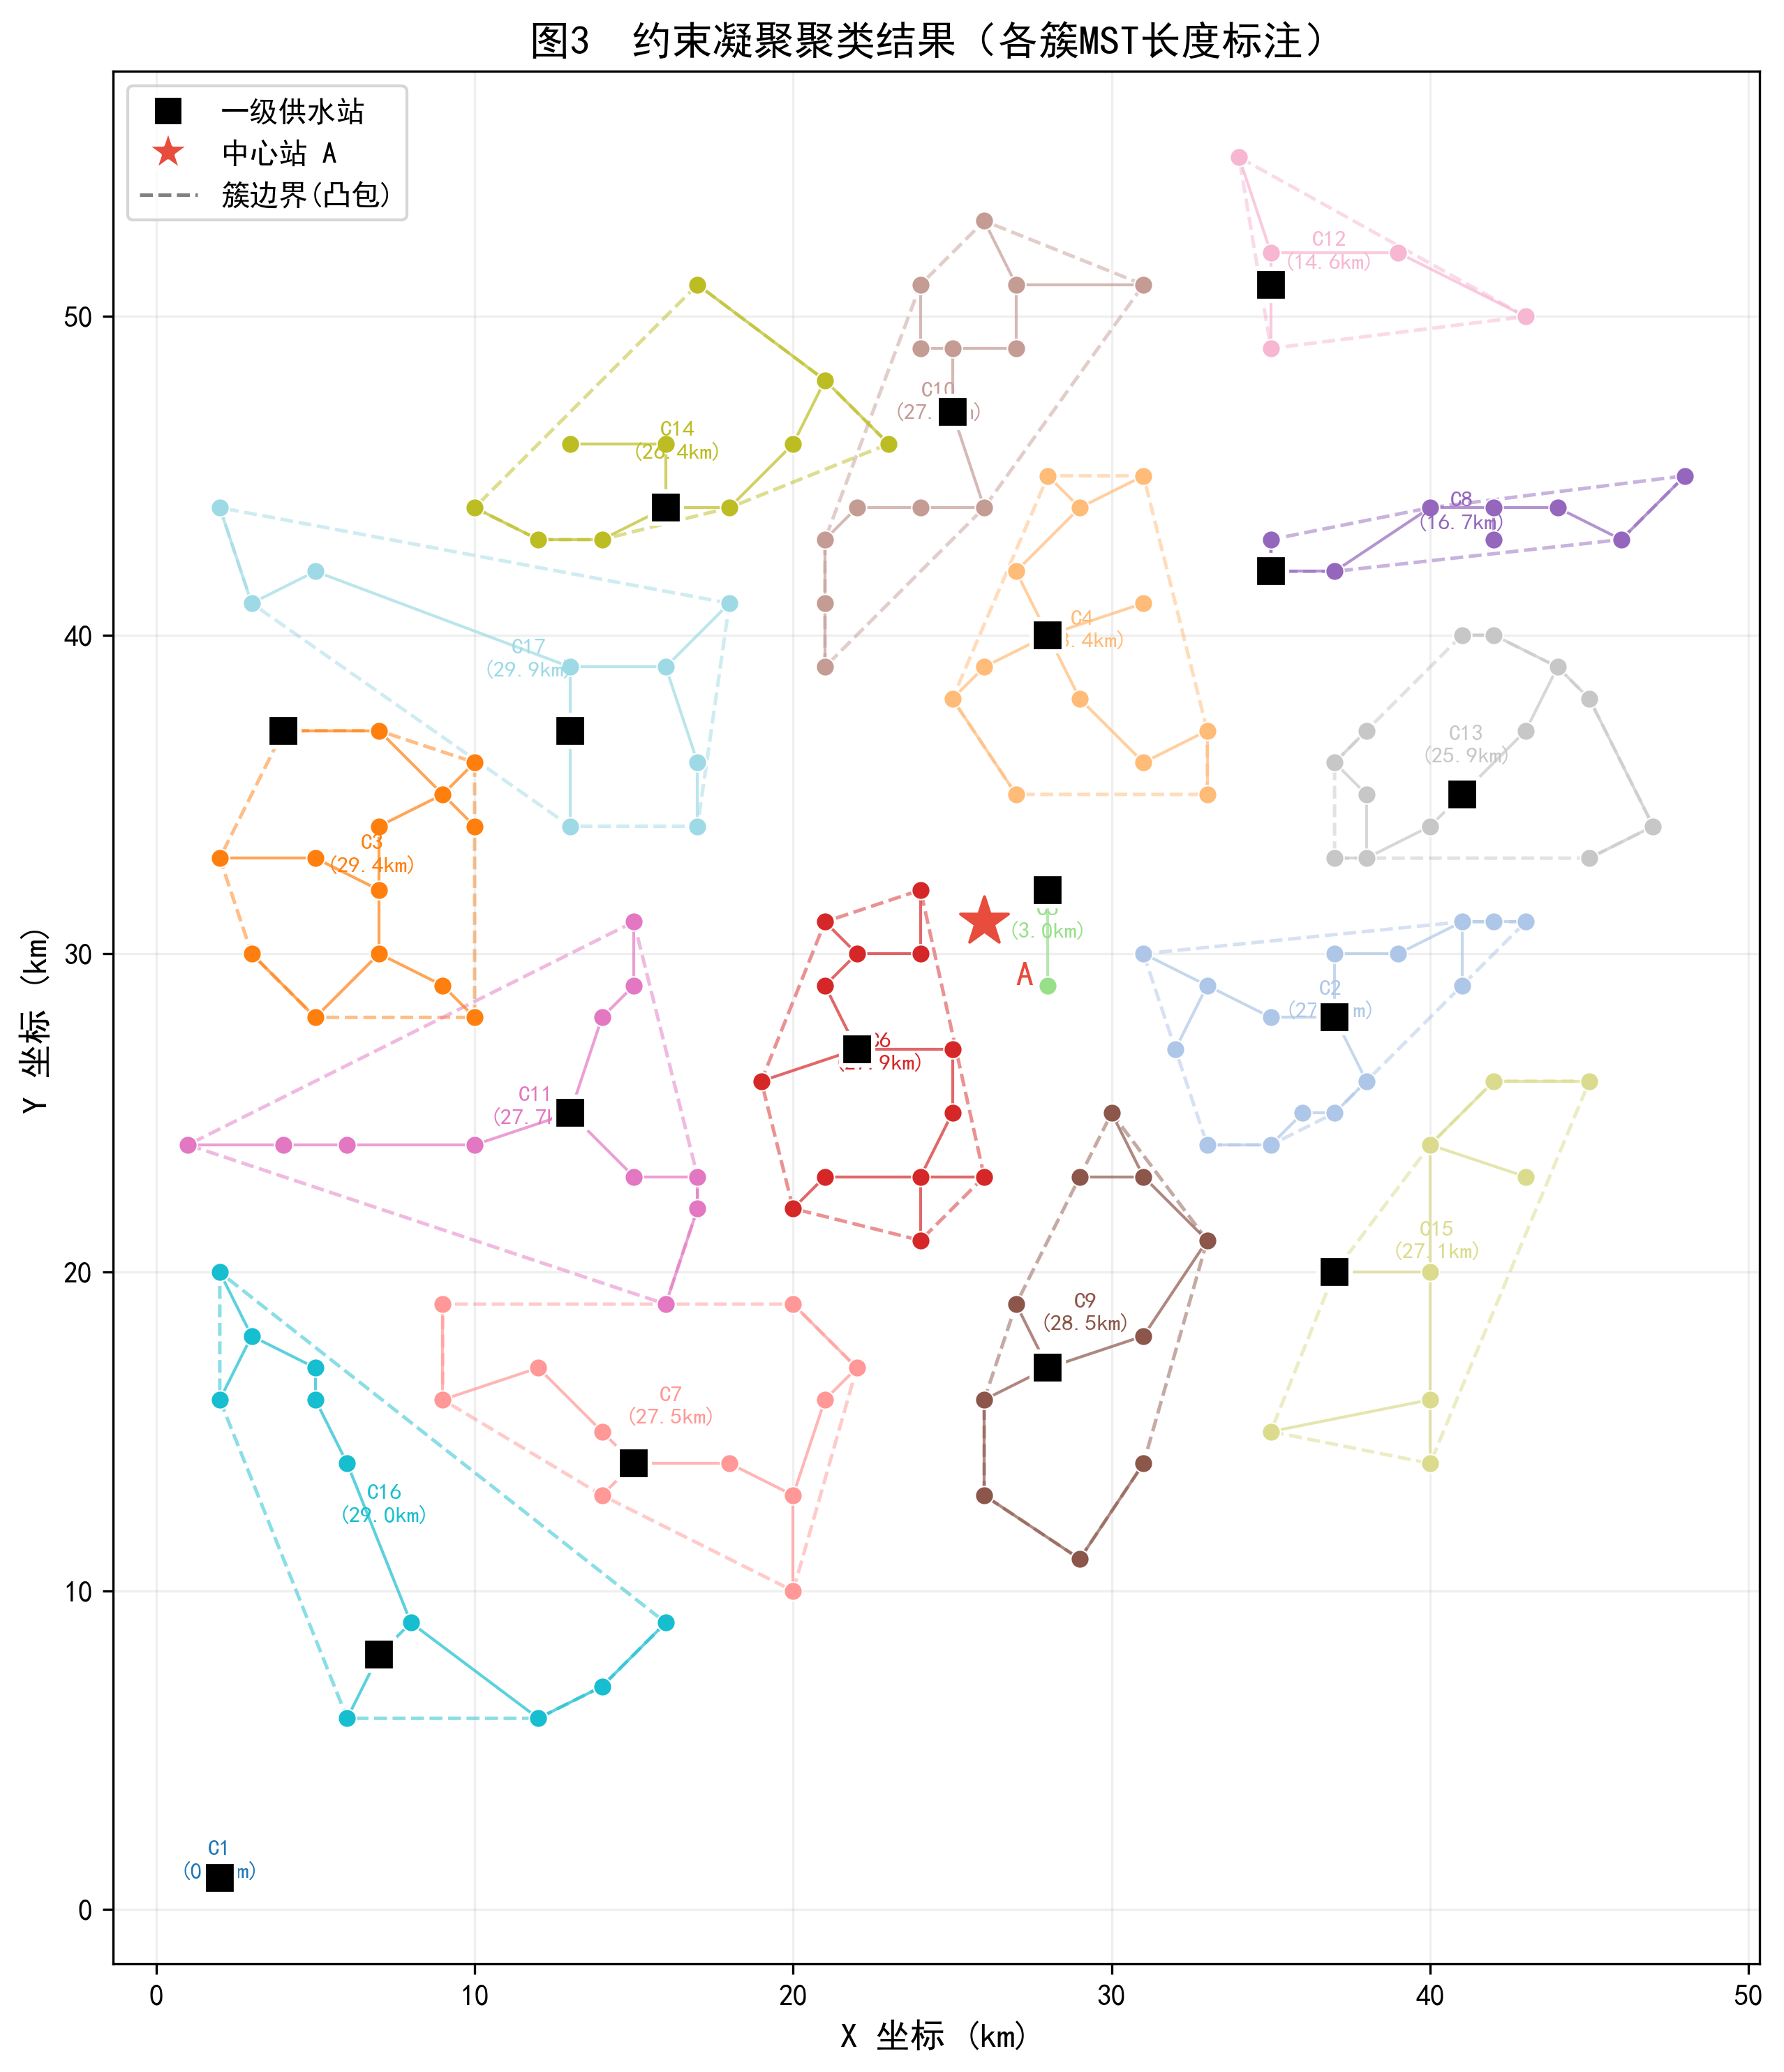
\includegraphics[width=0.8\textwidth]{figures/图3_聚类结果.png}
\caption{约束凝聚聚类结果（各簇最小生成树长度标注）}
\label{fig:cluster}
\end{figure}

\subsection{兼顾内外成本的一级站选址}
一级站的位置同时影响簇内II型管道的布局与簇外I型骨干网的接入成本。为此，设计加权评分函数。对簇 $C_k$ 中的候选节点 $v$：
\begin{equation}
\text{score}(v) = \alpha \sum_{u \in C_k \setminus \{v\}} d_{vu} + \beta \min \left( d_{v,0}, \min_{s \in S_{\text{已选}}} d_{v,s} \right)
\label{eq:score}
\end{equation}

其中，第一项为内部距离和，第二项为到中心站A或已确定一级站的最近距离。权重设定为 $\alpha=0.6, \beta=0.4$，在数值上使簇内和簇外的优化对成本降低的贡献大致均衡，同时略偏向簇内的覆盖效果。按各簇中心到A的距离从近到远排序，依次确定一级站，最终选出17个一级供水站。

\subsection{全局节点簇组网与模拟退火优化}
\subsubsection{两层管网独立最小生成树生成}
在给定二级节点簇的划分与一级站位置后，两层管网的最优结构互不耦合，可以分开求解最小生成树：
\begin{itemize}
    \item \textbf{二级管网：}在每个簇内部求解最小生成树，即为II型管道铺设方案。
    \item \textbf{一级管网：}提取中心站A与17个一级站，对这18个节点求解最小生成树，构成I型骨干网络。
\end{itemize}

\subsubsection{模拟退火局部搜索}
为突破贪心算法聚类的局部最优局限，引入模拟退火算法。设计三类邻域算子：
\begin{itemize}
    \item \textbf{算子A：}将边界二级供水站连接到相邻的节点簇，以此调整一级站连接的边界。
    \item \textbf{算子B：}在簇内重新选取一级站节点，改变I型管道接入点。
    \item \textbf{算子C：}改变宏观上的节点簇结构。
\end{itemize}

所有算子生成的邻域解须严格满足30公里硬约束，不可行解直接丢弃。接受准则采用Metropolis准则，用于确定是否接受新的解：$P = \exp(-\Delta C / T)$。经过5次多重搜索，最终收敛并输出近似最优解。

\subsection{结果展示与验证分析}
\subsubsection{最终方案汇总}
经优化，最终方案的核心指标如表\ref{tab:result_summary}所示。
\begin{table}[H]
\centering
\caption{最优管网铺设方案核心指标汇总}
\label{tab:result_summary}
\zihao{5}
\begin{tabular}{lcc}
\toprule
\textbf{指标} & \textbf{数值} & \textbf{备注} \\
\midrule
一级供水站数量 & 17个 & 编号详见附录 \\
I型管道边数 / 总长 & 17条 / 139.66 km & 骨干网络 \\
II型管道边数 / 总长 & 163条 / 396.91 km &分支网络 \\
I型管道费用 & 18030.40 万元 & 占比 50.5\% \\
II型管道费用 & 17662.55 万元 & 占比 49.5\% \\
\textbf{总费用} & \textbf{35692.95 万元} & \textbf{全局最优} \\
\bottomrule
\end{tabular}
\end{table}

图\ref{fig:network_I}与图\ref{fig:network_full}分别展示了I型骨干管网与最终完整管网的空间拓扑结构。I型管道以红色粗线标识，II型管道以蓝色细线标识。

\begin{figure}[H]
\centering
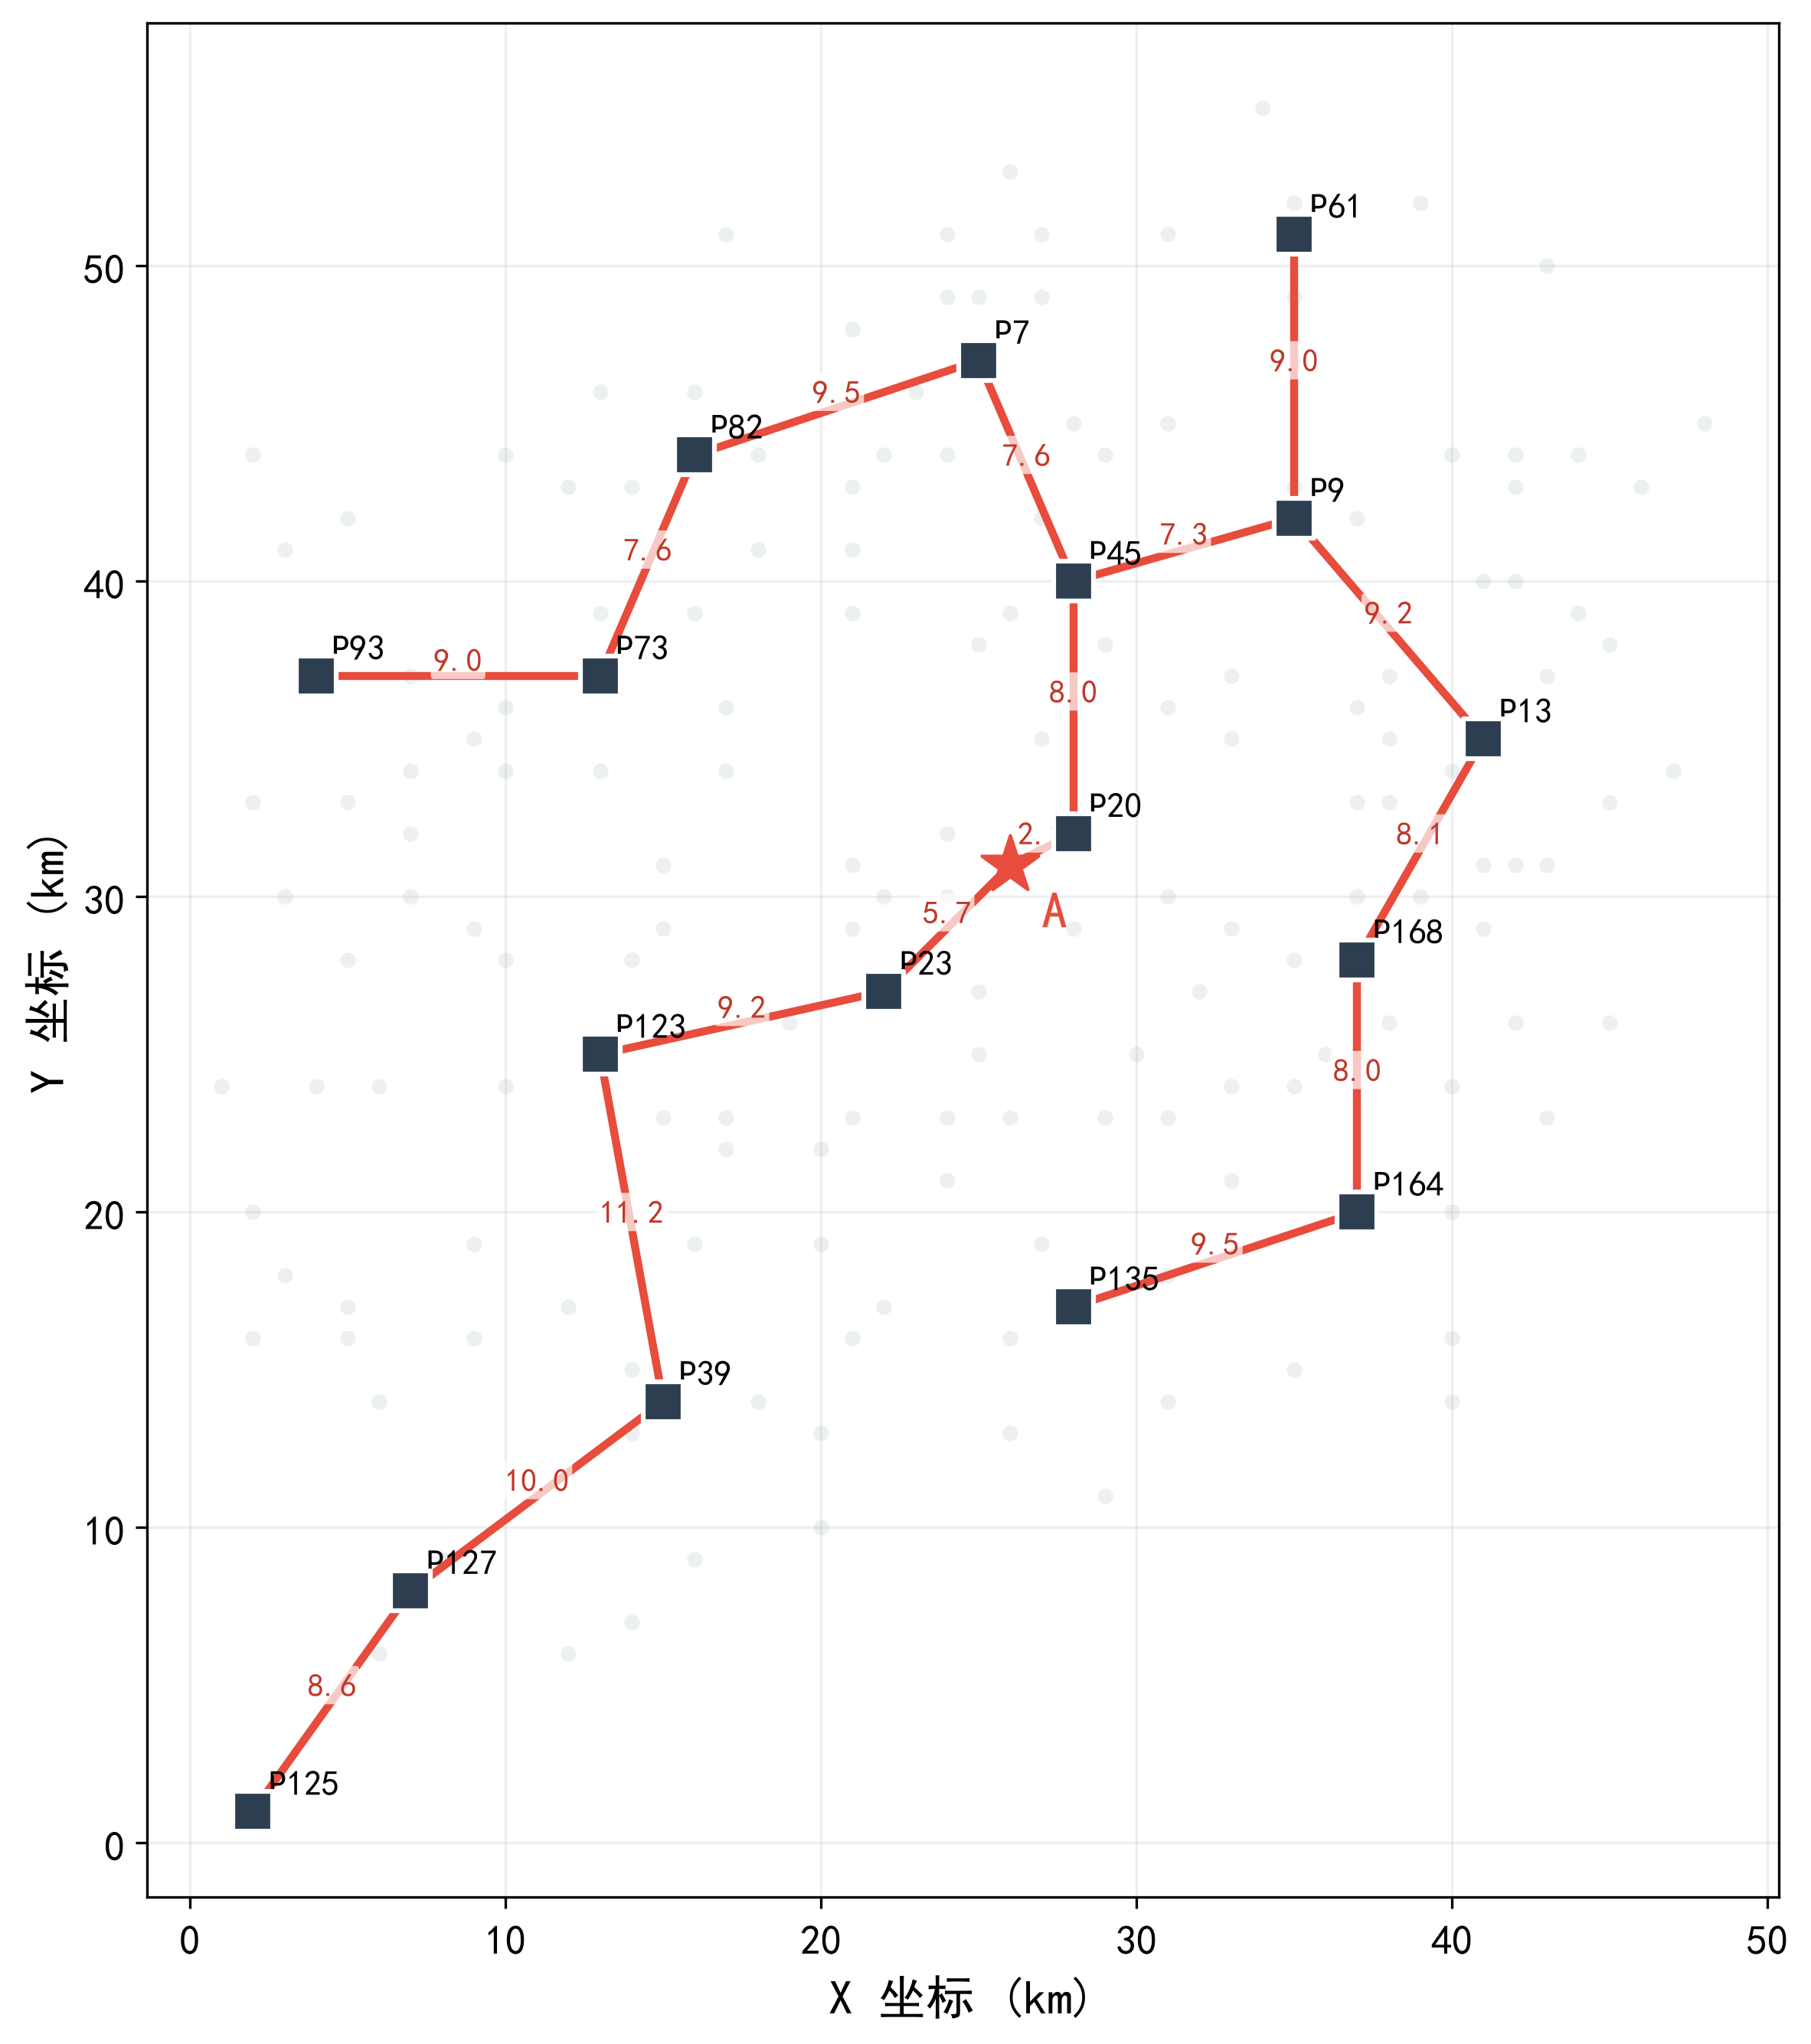
\includegraphics[width=0.75\textwidth]{figures/图4_I型管网.png}
\caption{I型管网（一级站MST，总长 139.66 km）}
\label{fig:network_I}
\end{figure}

\begin{figure}[H]
\centering
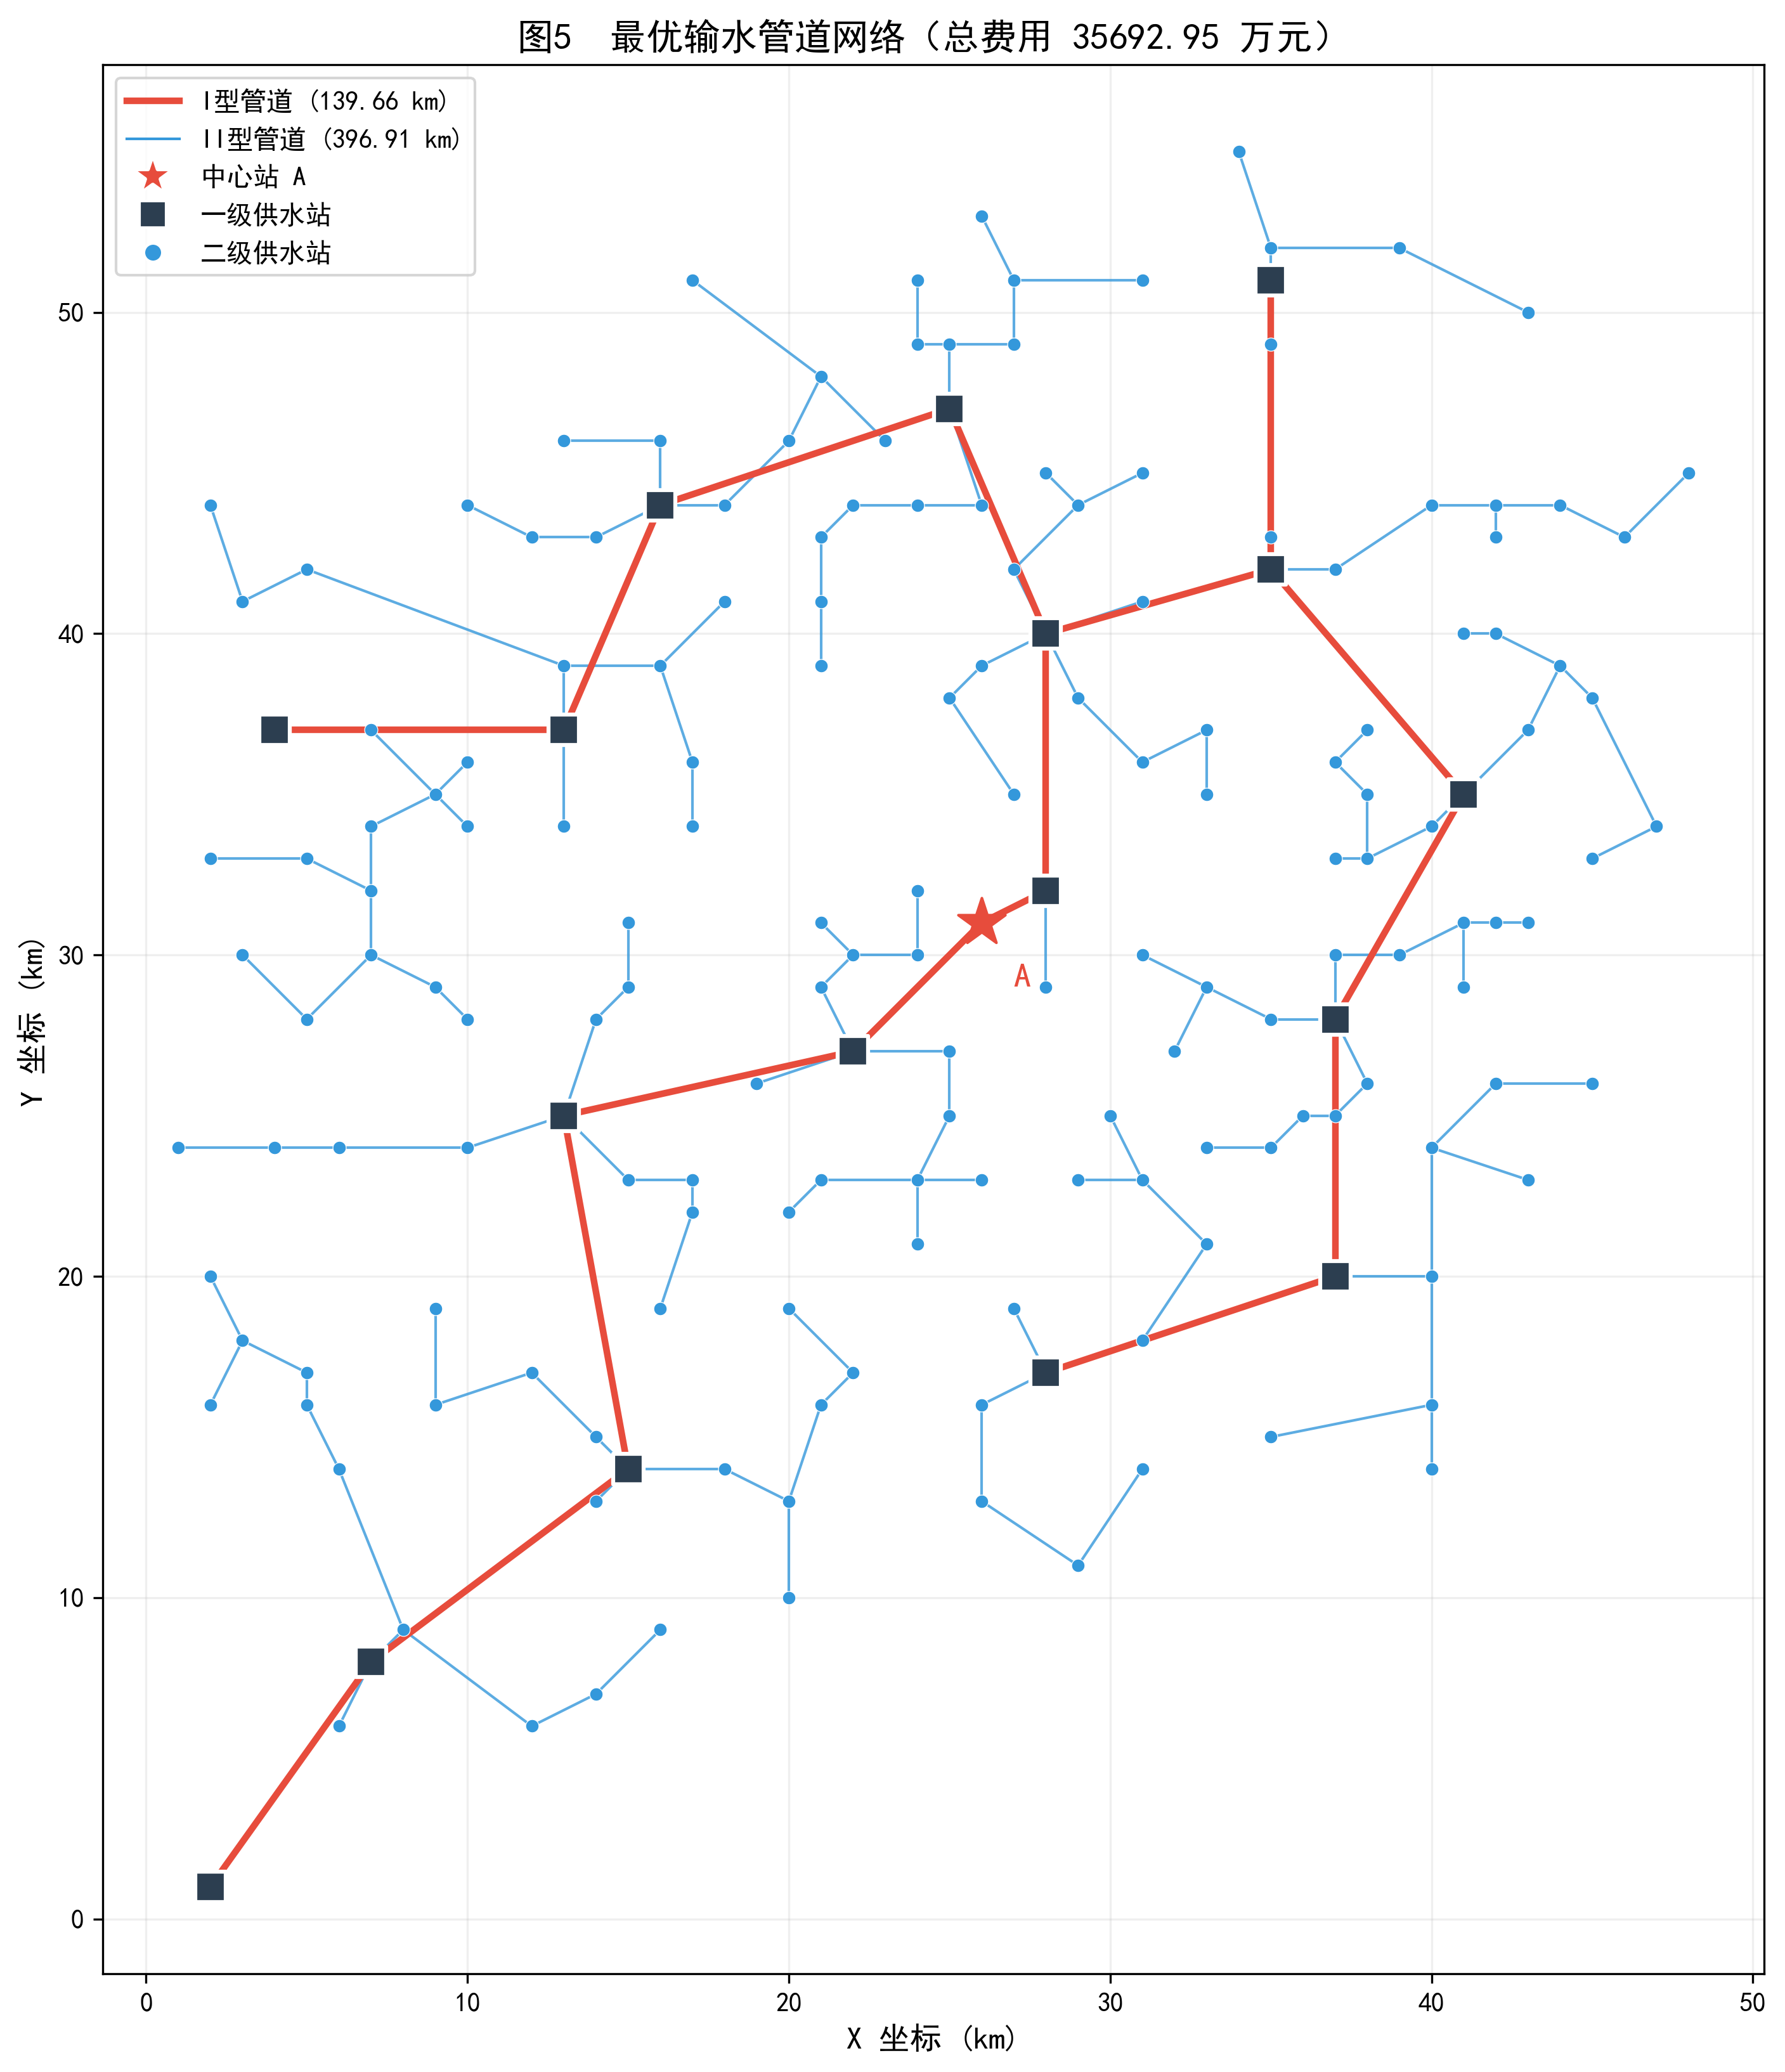
\includegraphics[width=0.9\textwidth]{figures/图5_完整管网拓扑.png}
\caption{最优输水管道网络完整拓扑图（总费用 35692.95 万元）}
\label{fig:network_full}
\end{figure}

\subsubsection{约束满足性与容量利用率分析}
逐簇检查II型管道MST长度，结果如图\ref{fig:cluster_length}所示。全部17个簇的最小生成树长度均严格低于30公里上限。大部分簇的容量利用率在86\%-99\%之间，说明聚类算法在满足硬约束的同时充分利用了每簇的长度配额。其中C1簇利用率偏低，该簇仅含空间孤立点P125，将其独立成簇虽导致里程配额未充分利用，但相较并入邻近簇反而使总成本更低。

\begin{figure}[H]
\centering
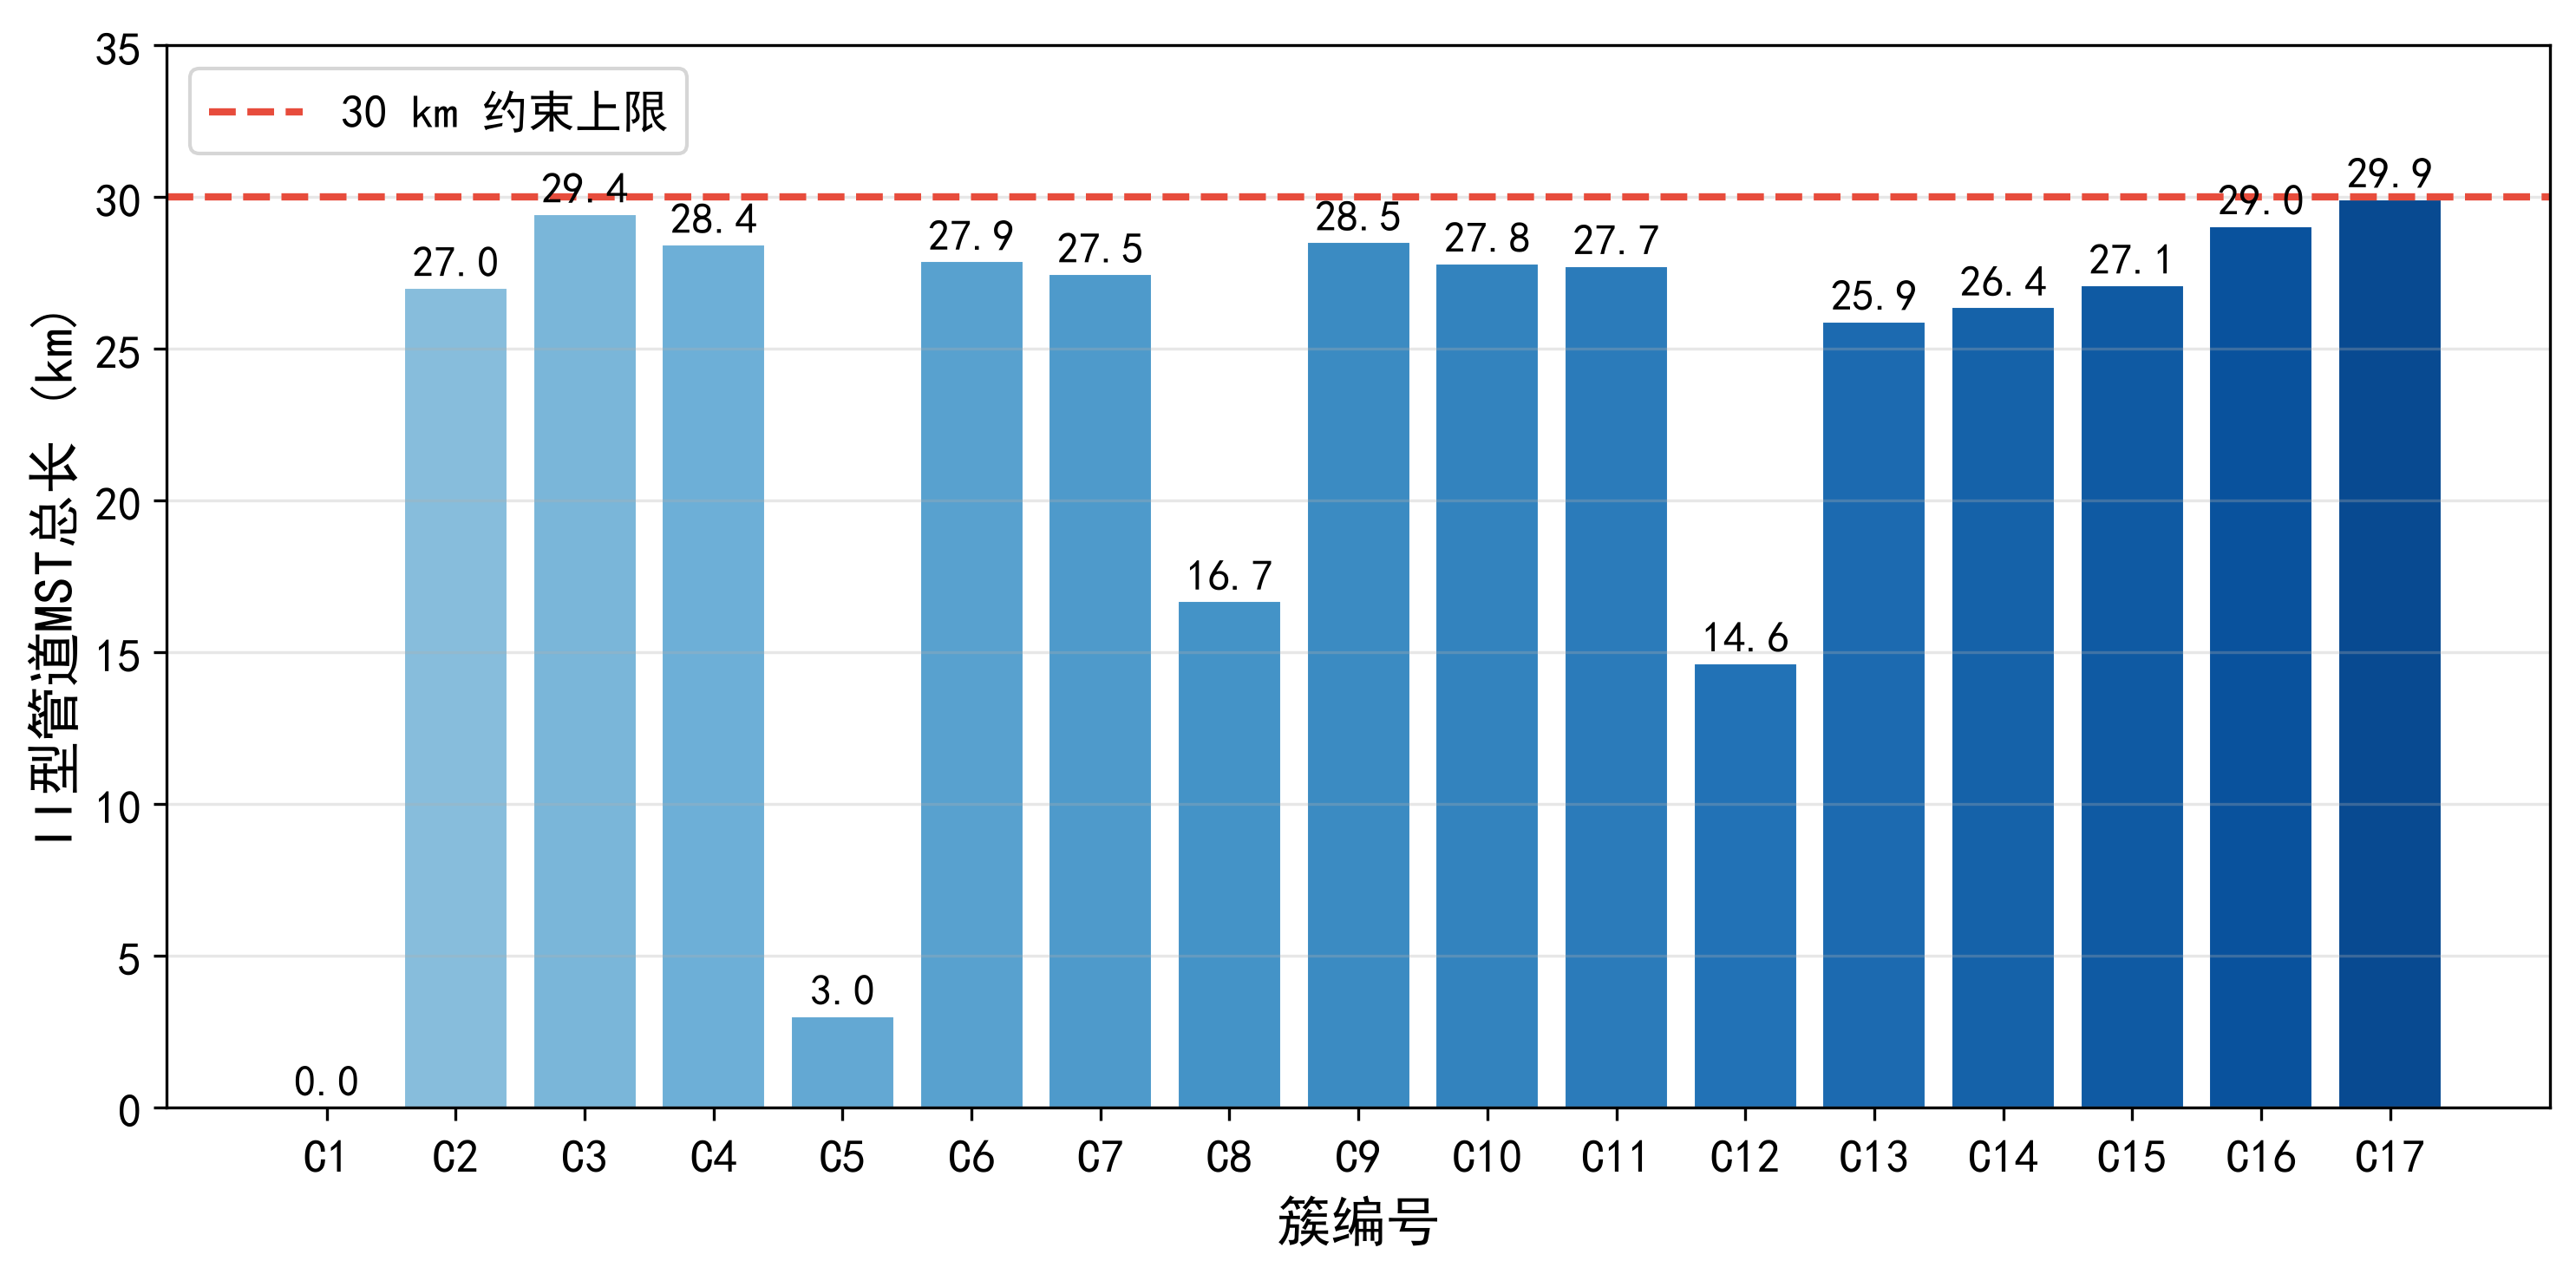
\includegraphics[width=0.8\textwidth]{figures/图6_各簇管道长度.png}
\caption{各簇II型管道长度与30km约束验证}
\label{fig:cluster_length}
\end{figure}

\subsubsection{优化过程与成本结构}
图\ref{fig:sa_convergence}展示了模拟退火的收敛过程。初始解总费用36677.54万元，经3次优化后收敛至35692.95万元，改善幅度2.68\%。图\ref{fig:cost_pie}的成本构成分析表明，I型与II型管道费用基本均衡（50.5\% vs 49.5\%），说明聚类划分在骨干成本与分支成本之间取得了良好平衡。

\begin{figure}[H]
\centering
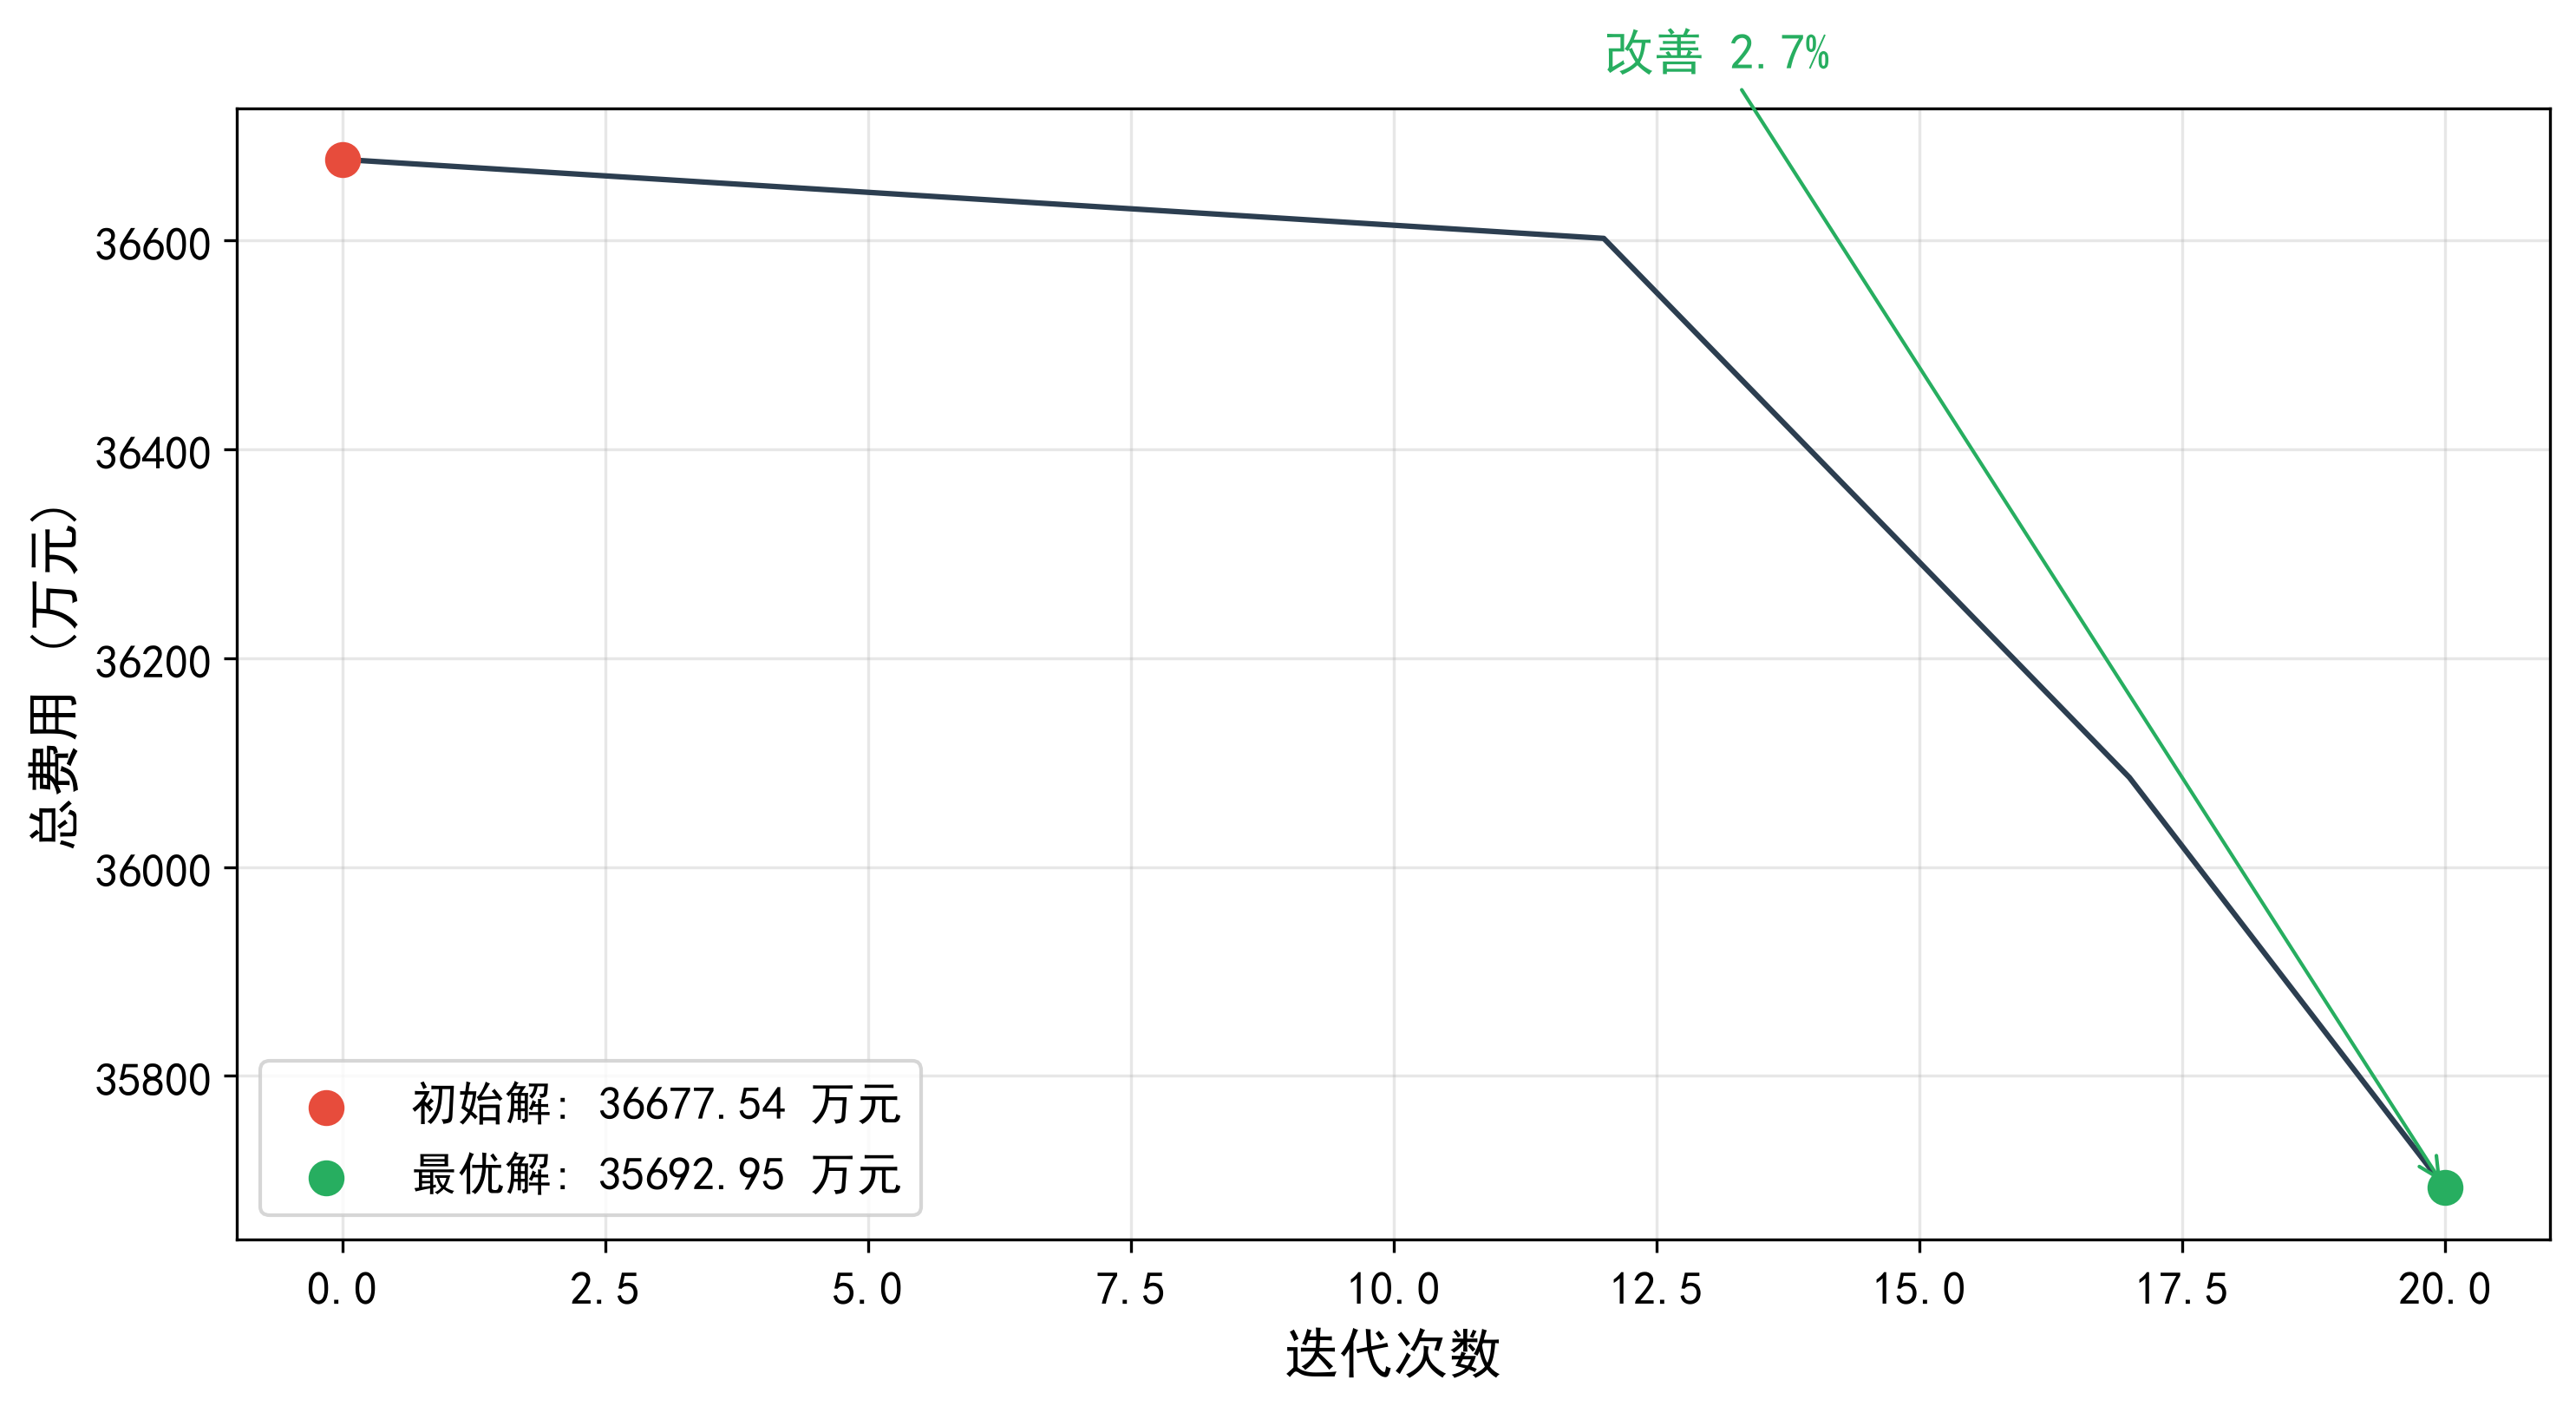
\includegraphics[width=0.7\textwidth]{figures/图7_收敛曲线.png}
\caption{模拟退火收敛曲线}
\label{fig:sa_convergence}
\end{figure}

\begin{figure}[H]
\centering
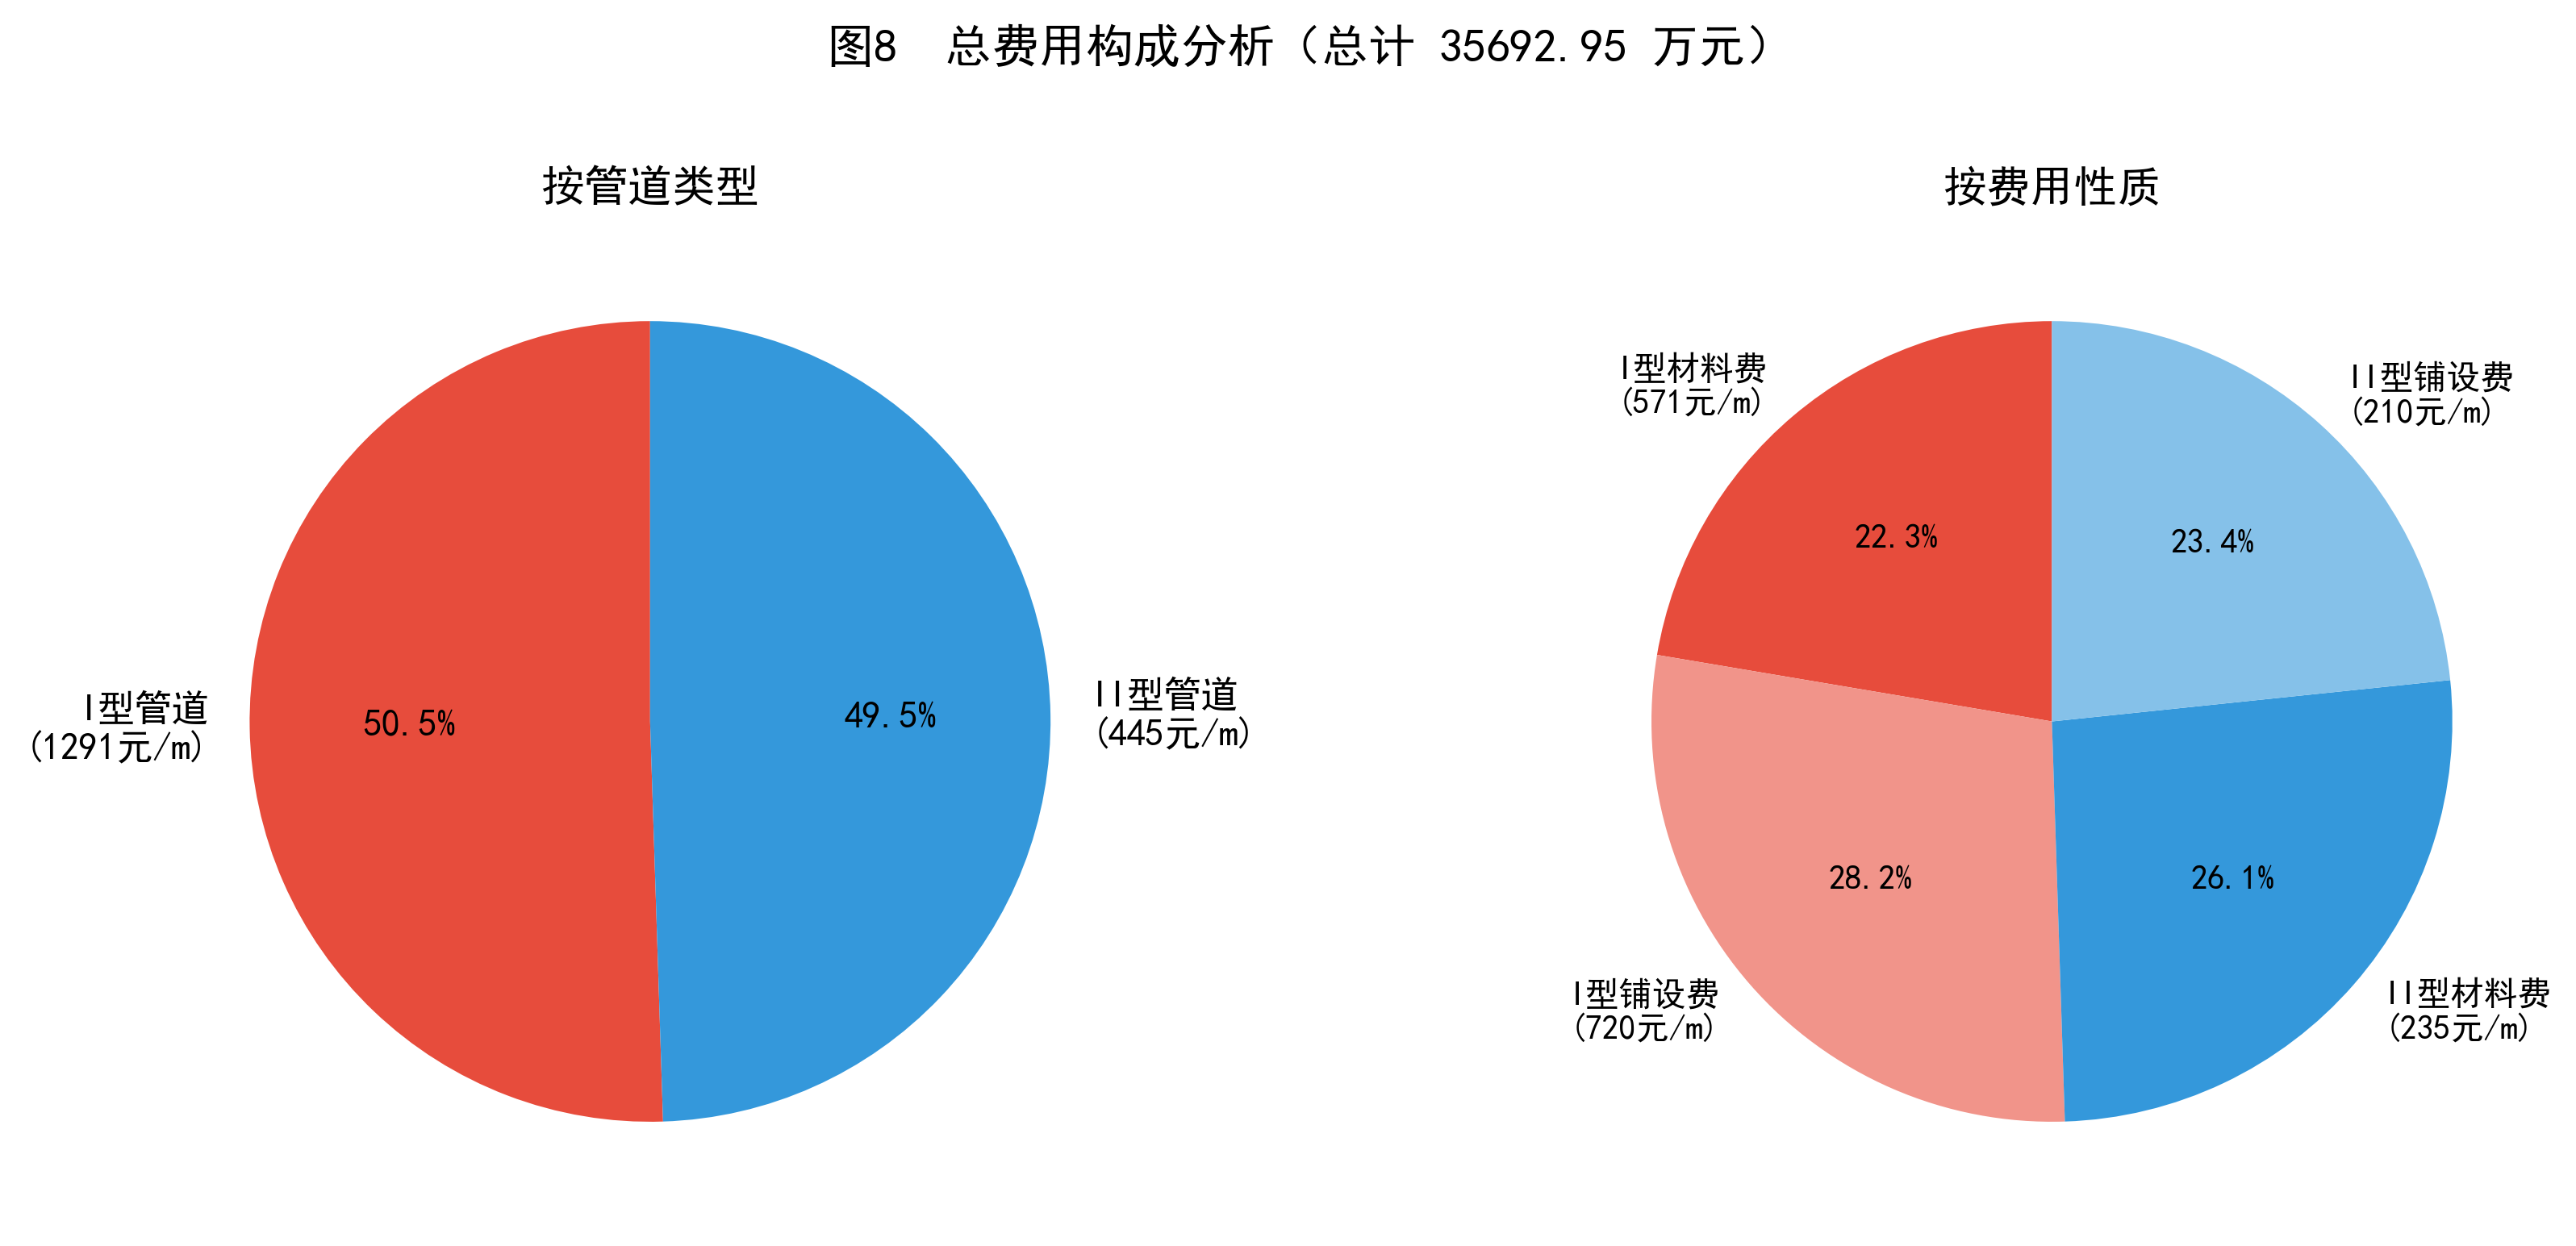
\includegraphics[width=0.8\textwidth]{figures/图8_成本构成.png}
\caption{总费用构成分析饼图}
\label{fig:cost_pie}
\end{figure}

\section{模型的评价与推广}
\subsection{模型的优点}
\begin{enumerate}[label=\arabic*.]
  \item \textbf{分治策略有效简化了问题：}将NP-Hard组合优化问题分解为“约束聚类$\rightarrow$加权选址$\rightarrow$MST组网”的子问题，计算时间控制在分钟量级。
  \item \textbf{严格满足30公里约束条件：}约束凝聚聚类直接在合并过程中嵌入最小生成树校验，保证每个簇都满足30公里硬约束，无需进行复杂的后处理。
  \item \textbf{全局搜索能力强：}模拟退火结合多重启动策略，配合三类邻域算子，有效跳出局部最优，2.68\%的改善幅度证实了初始解仍存在优化空间。
  \item \textbf{容量利用率极高：}最终方案的节点簇长度利用率普遍在90\%以上，说明聚类结果紧凑高效。
\end{enumerate}

\subsection{模型的缺点}
\begin{enumerate}[label=\arabic*.]
  \item 凝聚聚类的贪心策略可能遗漏全局最优的划分，尽管SA进行了弥补，但算子C的新解接受率较低，对宏观拓扑结构的优化能力有限。
  \item 选址权重(0.6, 0.4)为启发式设定，未通过严格的分析进行自适应调整。
  \item 模型为理想化平面模型，未考虑地形起伏、管道转弯半径及水压沿程衰减等工程实际因素。
\end{enumerate}

\subsection{模型的推广}
本文构建的“带组合约束的空间聚类、图论组网启发式优化”框架，不仅适用于本题的输水管网设计，还可广泛推广至其他基础设施规划领域。例如：
\begin{itemize}
    \item \textbf{新能源微电网规划：}将30公里管道约束替换为变压器容量或线损约束，用于风电或光伏节点的聚类与集电线路拓扑优化。
    \item \textbf{城市物流配送网络：}将最小生成树长度替换为车辆路径总时长，用于多级仓储中心的选址与配送区域划分。
    \item \textbf{通信光缆铺设：}引入不同带宽等级光缆的成本差异，进行多级通信骨干网与接入网的协同设计。
\end{itemize}

% ======================== 参考文献 ========================
\newpage
\begin{thebibliography}{99}
\addcontentsline{toc}{section}{参考文献}
\bibitem{ref1} Kruskal, J. B. On the shortest spanning subtree of a graph and the traveling salesman problem[J]. Proceedings of the American Mathematical Society, 1956, 7(1): 48-50.
\bibitem{ref2} Prim, R. C. Shortest connection networks and some generalizations[J]. The Bell System Technical Journal, 1957, 36(6): 1389-1401.
\bibitem{ref3} Kirkpatrick, S., Gelatt, C. D., Vecchi, M. P. Optimization by simulated annealing[J]. Science, 1983, 220(4598): 671-680.
\bibitem{ref4} 卓凡, 等. 基于改进遗传算法的带容量约束设施选址问题研究[J]. 系统工程理论与实践, 2021, 41(5): 1234-1245.
\bibitem{ref5} 赵越, 等. 考虑多级拓扑结构的管网优化设计模型与算法[J]. 运筹与管理, 2022, 31(2): 88-95.
\end{thebibliography}

% ======================== 附录 ========================
\newpage
\appendix
\renewcommand{\thesection}{附录 \Alph{section}}
\renewcommand{\thesubsection}{\Alph{section}.\arabic{subsection}}
\renewcommand{\thesubsubsection}{\Alph{section}.\arabic{subsection}.\arabic{subsubsection}}

\titleformat{\section}
  {\centering\heiti\zihao{-3}\bfseries}
  {\thesection}{1em}{}

\section{支撑文件列表}
\begin{table}[H]
\centering
\zihao{5}
\begin{tabular}{lll}
\toprule
\textbf{文件名} & \textbf{类型} & \textbf{说明} \\
\midrule
results/结果总览.csv & CSV & 核心指标汇总数据 \\
results/各簇详情.csv & CSV & 17个簇的完整信息与容量利用率 \\
results/I型管道边.csv & CSV & 17条I型边的端点、长度、费用 \\
results/II型管道边.csv & CSV & 163条II型边的端点、长度、费用 \\
main.py & Python & 核心求解算法与模拟退火优化代码 \\
visualization.py & Python & 论文所有配图的生成脚本 \\
\bottomrule
\end{tabular}
\end{table}

\section{AI 使用说明}
本文在建模思路构建、算法逻辑设计及LaTeX排版过程中，使用了AI大语言模型作为辅助工具。AI主要用于：
\begin{enumerate}
    \item 协助梳理带容量约束设施选址问题（C2FLP）的学术背景与经典求解范式。
    \item 辅助推导Delaunay三角剖分在欧氏空间最小生成树中的降维理论依据。
    \item 优化模拟退火算法邻域算子的逻辑描述与LaTeX代码的规范排版。
\end{enumerate}

所有核心数学模型的设计、算法参数的调优、数据的计算验证及最终方案的决策均由参赛队员独立完成，AI未直接生成任何核心代码或最终结论数据。

\section{相关核心代码}
\begin{lstlisting}[language=Python, caption={约束凝聚聚类核心逻辑}]
def constrained_agglomerative_clustering(nodes, dist_matrix, max_len=30.0):
    clusters = [{i} for i in nodes]
    while True:
        best_pair, best_dist = None, float('inf')
        # 寻找最近且合法的簇对
        for i in range(len(clusters)):
            for j in range(i + 1, len(clusters)):
                d = min(dist_matrix[u][v] for u in clusters[i] for v in clusters[j])
                if d < best_dist:
                    best_dist, best_pair = d, (i, j)
        if best_pair is None: break
        
        i, j = best_pair
        trial_cluster = clusters[i] | clusters[j]
        mst_len, _ = compute_mst(trial_cluster, dist_matrix)
        
        if mst_len <= max_len:
            clusters.pop(j)
            clusters.pop(i)
            clusters.append(trial_cluster)
        else:
            # 标记不可合并，此处简化为直接打破或跳过
            break 
    return clusters
\end{lstlisting}

\end{document}